\documentclass[12pt,]{article}
\usepackage{graphicx}
\usepackage{subcaption}
\usepackage{float}
\graphicspath{{Images/}}
\usepackage{amsmath}
\numberwithin{figure}{section}
\usepackage{multirow}
%\usepackage{wrapfig}

\begin{document}
\tableofcontents
\newpage
\listoffigures
\newpage
\listoftables
\newpage


\section{Introduction}
The concept of remote monitoring and control (R\&C), has its roots like many technological advancements in the arms race during World War II. Its first implementation sought to create unmanned aircraft capable of delivering greater payloads at longer distances. Fast forward to 1960's the first successful use of remote monitoring in a medical field was the need for medical testing and care in a remote location such as outer space. Kaiser Foundation International (KFI), tackled this problem and became a major (\$1.8 million in the 1970's adjusted for inflation this equals about \$11.5 million today) subcontractor to the Lockheed Missiles and Space Company (LMSC) to help design, develop and test a ground based remote health care delivery system. "The ground-based test unit will be installed at a sparsely populated site on earth to provide medical care to local residents. Trained physicians’ assistants will employ the unit to transmit medical information on residents of the area to physicians at an established facility many miles from the remote site. If the test program is successful, it may provide system technology to improve health care and medical services to remote areas on earth. Part of a four year NASA sponsored program, this concept, as applied to a remote area on earth, will be evaluated by NASA for possible use in advanced, long-duration, manned space missions." \cite{KFI} . Figure~\ref{fig:1} on page~\pageref{fig:1} shows the logo of the Space Technology Applied to Rural Papago Advanced Health Care (STARPAHC) logo.
\begin{figure}[H]
  	\begin{center}
    	
\includegraphics[width=0.8\textwidth]{1}
  	\end{center}
  	\caption{Space Technology Applied to Rural Papago Advanced Health Care \cite{KFI}}
	\label{fig:1}
\end{figure}
But there were still many barriers standing in the way of widespread adoption of M\&C tools in healthcare. Some of the main challenges include: data transfer rates,lack of broadband infrastructure, financial and technological to name a few, that made it difficult to implement on a civilian scale. True civilian scale implementation began in the last decade (2010's), in America with the 'Connecting America: The National Broadband Plan' that aimed to "assist in the proliferation and improvement of broadband networks across the United States." \cite{FCC}. With the technological advancements since then, it is now more financially feasible to adopt a telemedicical technology  due to a well developed, fast (data rate transfer) and cheap broadband infrastructure, as well as smaller, faster and more power efficient micro-controller-sensor integrated circuits.
\subsection{Project aims}
\textbf{The aim of the project is to:}
\begin{itemize}
	\item[1] Design and program a wearable device for:
	\begin{itemize}
		\item Collecting Electrocardiography (ECG) data,
		\item Sensing wearers physical activity 					(Pedometer).
	\end{itemize}
	The device must then be able to send the data to a 			remote database.
	\item[2] Design and program the database to store the 		ECG and Pedometer data.
	\item[3] Build a website that is able to display the 		data. 
\end{itemize}
Figure~\ref{fig:2} on page~\pageref{fig:2} shows a simplified flowchart of the possible data flow sequence. For the detailed flow chart see Figure~\ref{fig:12} on page~\pageref{fig:12}.
\begin{figure}[h]
	\centering
    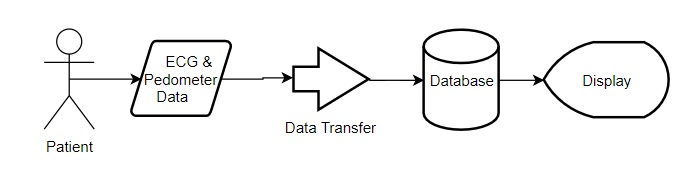
\includegraphics[width=0.8\textwidth]{2}
    \caption{A simplified flow chart of the project aim}
    \label{fig:2}
\end{figure}
\newpage
\section{Analysis and design}
In a lot of cases today, the need for patients to stay in hospital for long periods of time, is due to the need to monitor their biological signals as well as well-being. This is done to provide a safe environment for their recovery after treatment, or in case a diagnosis could not be made, to monitor them until the patient is deemed safe to discharge. This is especially true for older patients. The use of mobile sensors combined with remote monitoring would enable these patients to be discharged earlier compared to standard discharge time. This in turn would free up hospital space. Another benefit of this would be a substantial decrease in the cost of health care per a patient.
Another advantage of remote monitoring in healthcare is the possibility of implementation and use of a intelligent algorithms, which would continuously scan the data for anomalies in patients vital signs and identification of everyday routines and warning in case an out of ordinary event has been identified.\\
\\
Recent advancements in technology facilitate the development of R\&C even more. The use of smart sensors, which combine integrated circuits with sensing materials have already revolutionised many scientific, commercial and engineering fields. This is due to the fact that microprocessors have been getting smaller, faster and more power efficient with time, coupled with wireless connectivity where high data rates are available seemingly everywhere.
\subsection{Existing implementations}
As this concept is not new, there are a lot of companies that have already developed and created different solutions each with unique pros and cons. They find use both as private client based products as well as hospital provided services for better care and more efficient work flow. Some of the leading remote monitoring solution providers are:
\begin{itemize}
\item Biotronik Home Monitoring,
\item Boston Scientific LATITUDE NXT,
\item A\&D Medical, Wellness Connected,
\item GE Healthcare, Apex Pro CH.
\end{itemize}
\subsubsection{Biotronik Home Monitoring}
Biotronik Home Monitoring is a pioneering and first in class, remote cardiac monitoring system. Designed to maximise patient comfort while reducing patients effort, it sends data daily. Continuous cardiac device data is sent to the personal patient device, which in turn forwards the information to the Home Monitoring Service Center (HMSC). Furthermore HMSC allows physicians to safely review cardiac functions as well as sending alerts about relevant changes in patient health and the device’s status. This allows for the continuous monitoring of both the patient’s condition and the device. Figure~\ref{fig:3} on page~\pageref{fig:3} shows the company's logo, with their trademark slogan "excellence for life".
\begin{figure}[h]
  	\begin{center}
    	
\includegraphics[width=0.8\textwidth]{3}
  	\end{center}
  	\caption{Biotronik logo \cite{BIO}}
	\label{fig:3}
\end{figure}
\subsubsection{Boston Scientific LATITUDE NXT}
Boston Scientific LATITUDE NXT is a in-home monitoring system allowing physicians to monitor connected devices between care visits. These devices send data at scheduled time, some of the devices that can connect to the LATITUDE NXT include: blood pressure monitors, cardiac monitors, weight scales, pacemakers and other healthcare devices.This products enables patients to plug-in the Communicator to the all ready existing analogue and digital phone lines, allowing the Communicator to connect to the LATITUDE system. In case the Communicator is not compatible with the phone line, additional equipment is required to connect via internet or cellular network. The connector is hands-free, meaning that it does not require patient intervention to send data and that it is done automatically. The LATITUDE NXT system is designed to improve clinic efficiency as well as provide a higher level of care for device patients. The company also developed an App that allows clinicians a read-only access to see LATITUDE NXT system patient data from an iPhone. Figure~\ref{fig:4} on page~\pageref{fig:4} shows the LATITUDE Communicator.
\begin{figure}[h]
  	\begin{center}
    	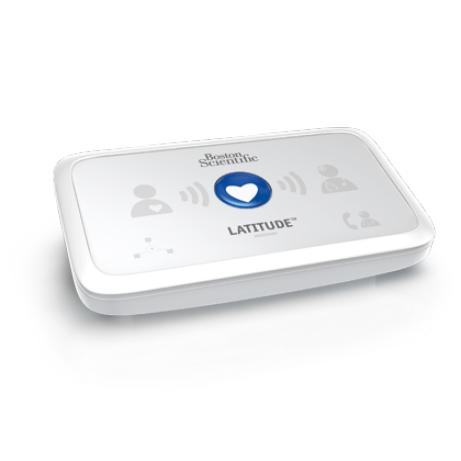
\includegraphics[width=0.8\textwidth]{4}
  	\end{center}
  	\caption{LATITUDE Wireless Communicator \cite{BOS}}
	\label{fig:4}
\end{figure}
\subsubsection{A\&D Medical, Wellness Connected}
Wellness Connected is an App that is simple and easy-to-use available for both Android and iOS users. It allows clients to manage their health and wellness by monitoring their key health metrics. From blood pressure, heart rate, weight to activity, calorie usage and sleep patterns. The App allows the client to better understand their current health state and allows for setting goals and charts the clients progress. The app also allows the user to share their current progress with family and even physicians. The App is free on both AppStore and Google play but it requires the A\&D Medical connected devices to gather data. The product range includes:
\begin{itemize}
\item[a] Deluxe Connected Weight Scale see figure~\ref{fig:8} on page~\pageref{fig:8},
\item[b] Deluxe Connected Blood Pressure Monitor see figure~\ref{fig:30} on page~\pageref{fig:30},
\item[c] Lifetrak Move Connected Activity Tracker see figure~\ref{fig:31} on page~\pageref{fig:31},
\item[d] Lifetrak Zone Connected Activity and Sleep Tracker see figure~\ref{fig:32} on page~\pageref{fig:32}.
\end{itemize}
This allows the user to tailor the data collected about them to their own preference and need but requires the user to interact with all the separate devices, which can be inconvenient.
\begin{figure}[h]
  	\begin{center}
    	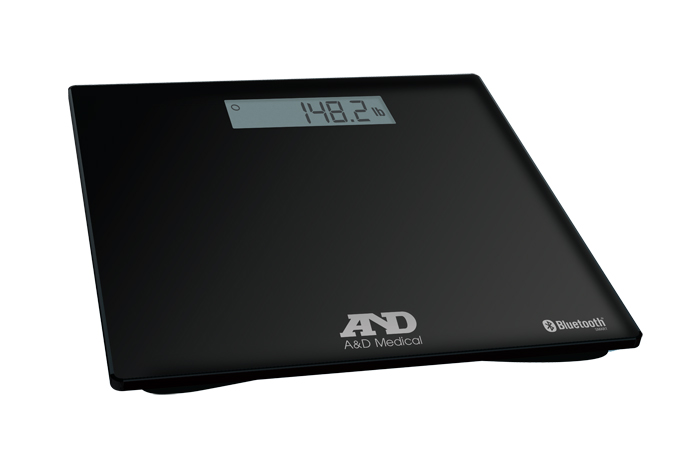
\includegraphics[width=0.8\textwidth]{5}
   	\end{center}
  	\caption{Weight Scale \cite{AND}}
	\label{fig:8}
\end{figure}
\begin{figure}
	\begin{center}
		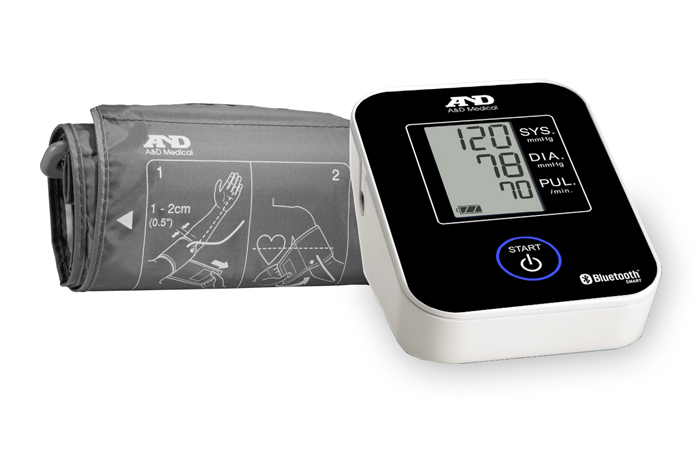
\includegraphics[width=0.8\textwidth]{6}
	\end{center}
    \caption{Blood Pressure Monitor \cite{AND}}
	\label{fig:30}
\end{figure}
\begin{figure}
	\begin{center}
		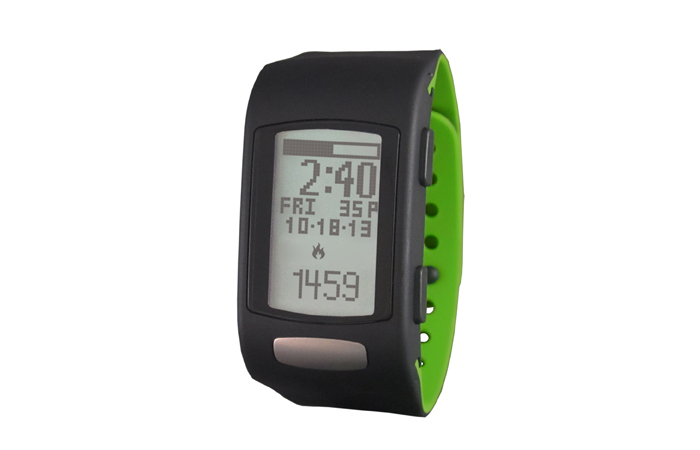
\includegraphics[width=0.8\textwidth]{7}
	\end{center}
    \caption{Activity Tracker \cite{AND}}
	\label{fig:31}
\end{figure}
\begin{figure}
	\begin{center}
		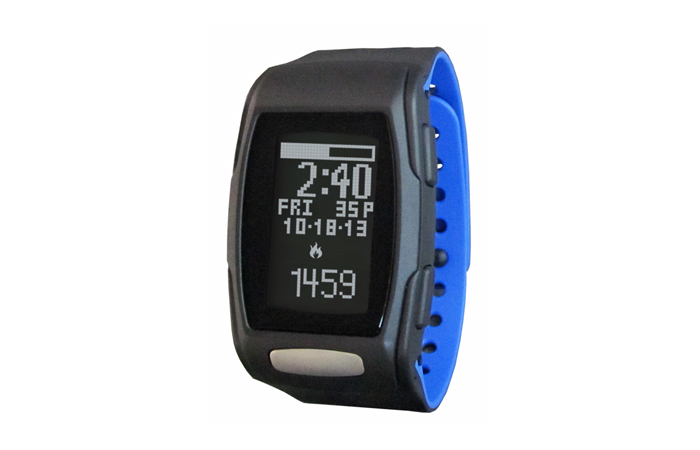
\includegraphics[width=0.8\textwidth]{8}
	\end{center}
    \caption{Activity and Sleep Tracker \cite{AND}}
	\label{fig:32}
\end{figure}
\subsubsection{GE Healthcare, Apex Pro CH}
Apex Pro CH is a medical system offered by GE Healthcare. "ApexPro CH telemetry offers a highly flexible telemetry system to meet the current and future telemetry needs of growing hospitals" \cite{GEH}. The ApexPro monitoring allows for centralised as well as decentralised use. Because the data is accessible throughout the whole facility (Hospital), patients can migrate throughout the organisation while being monitored. Figure~\ref{fig:9} on page~\pageref{fig:9} shows one of many GE Healthcare products compatible with their Apex Pro CH platform in this case the ApexPro FH.
\begin{figure}[h]
  	\begin{center}
    	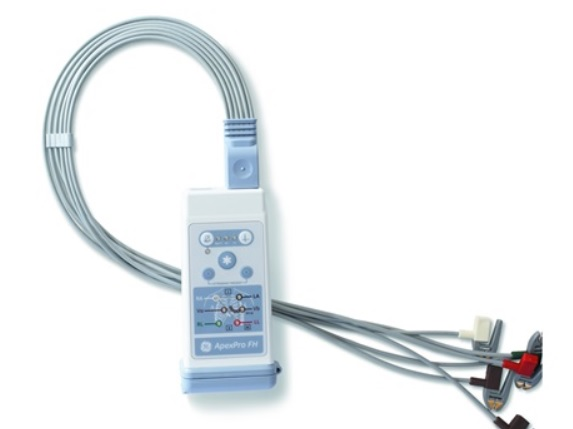
\includegraphics[width=0.8\textwidth]{9}
  	\end{center}
  	\caption{ApexPro FH Telemetry System \cite{GEH}}
	\label{fig:9}
\end{figure}
\subsection{User expectations}
The final design should require as little interaction from the user as possible, and be simple to set up with regards to the wearable device see figure~\ref{fig:28} on page~\pageref{fig:28}. The device should also be capable of wireless communication. And with regards to the viewing data website, it should be intuitive for the user to interact.
\begin{figure}[h]
  	\begin{center}
    	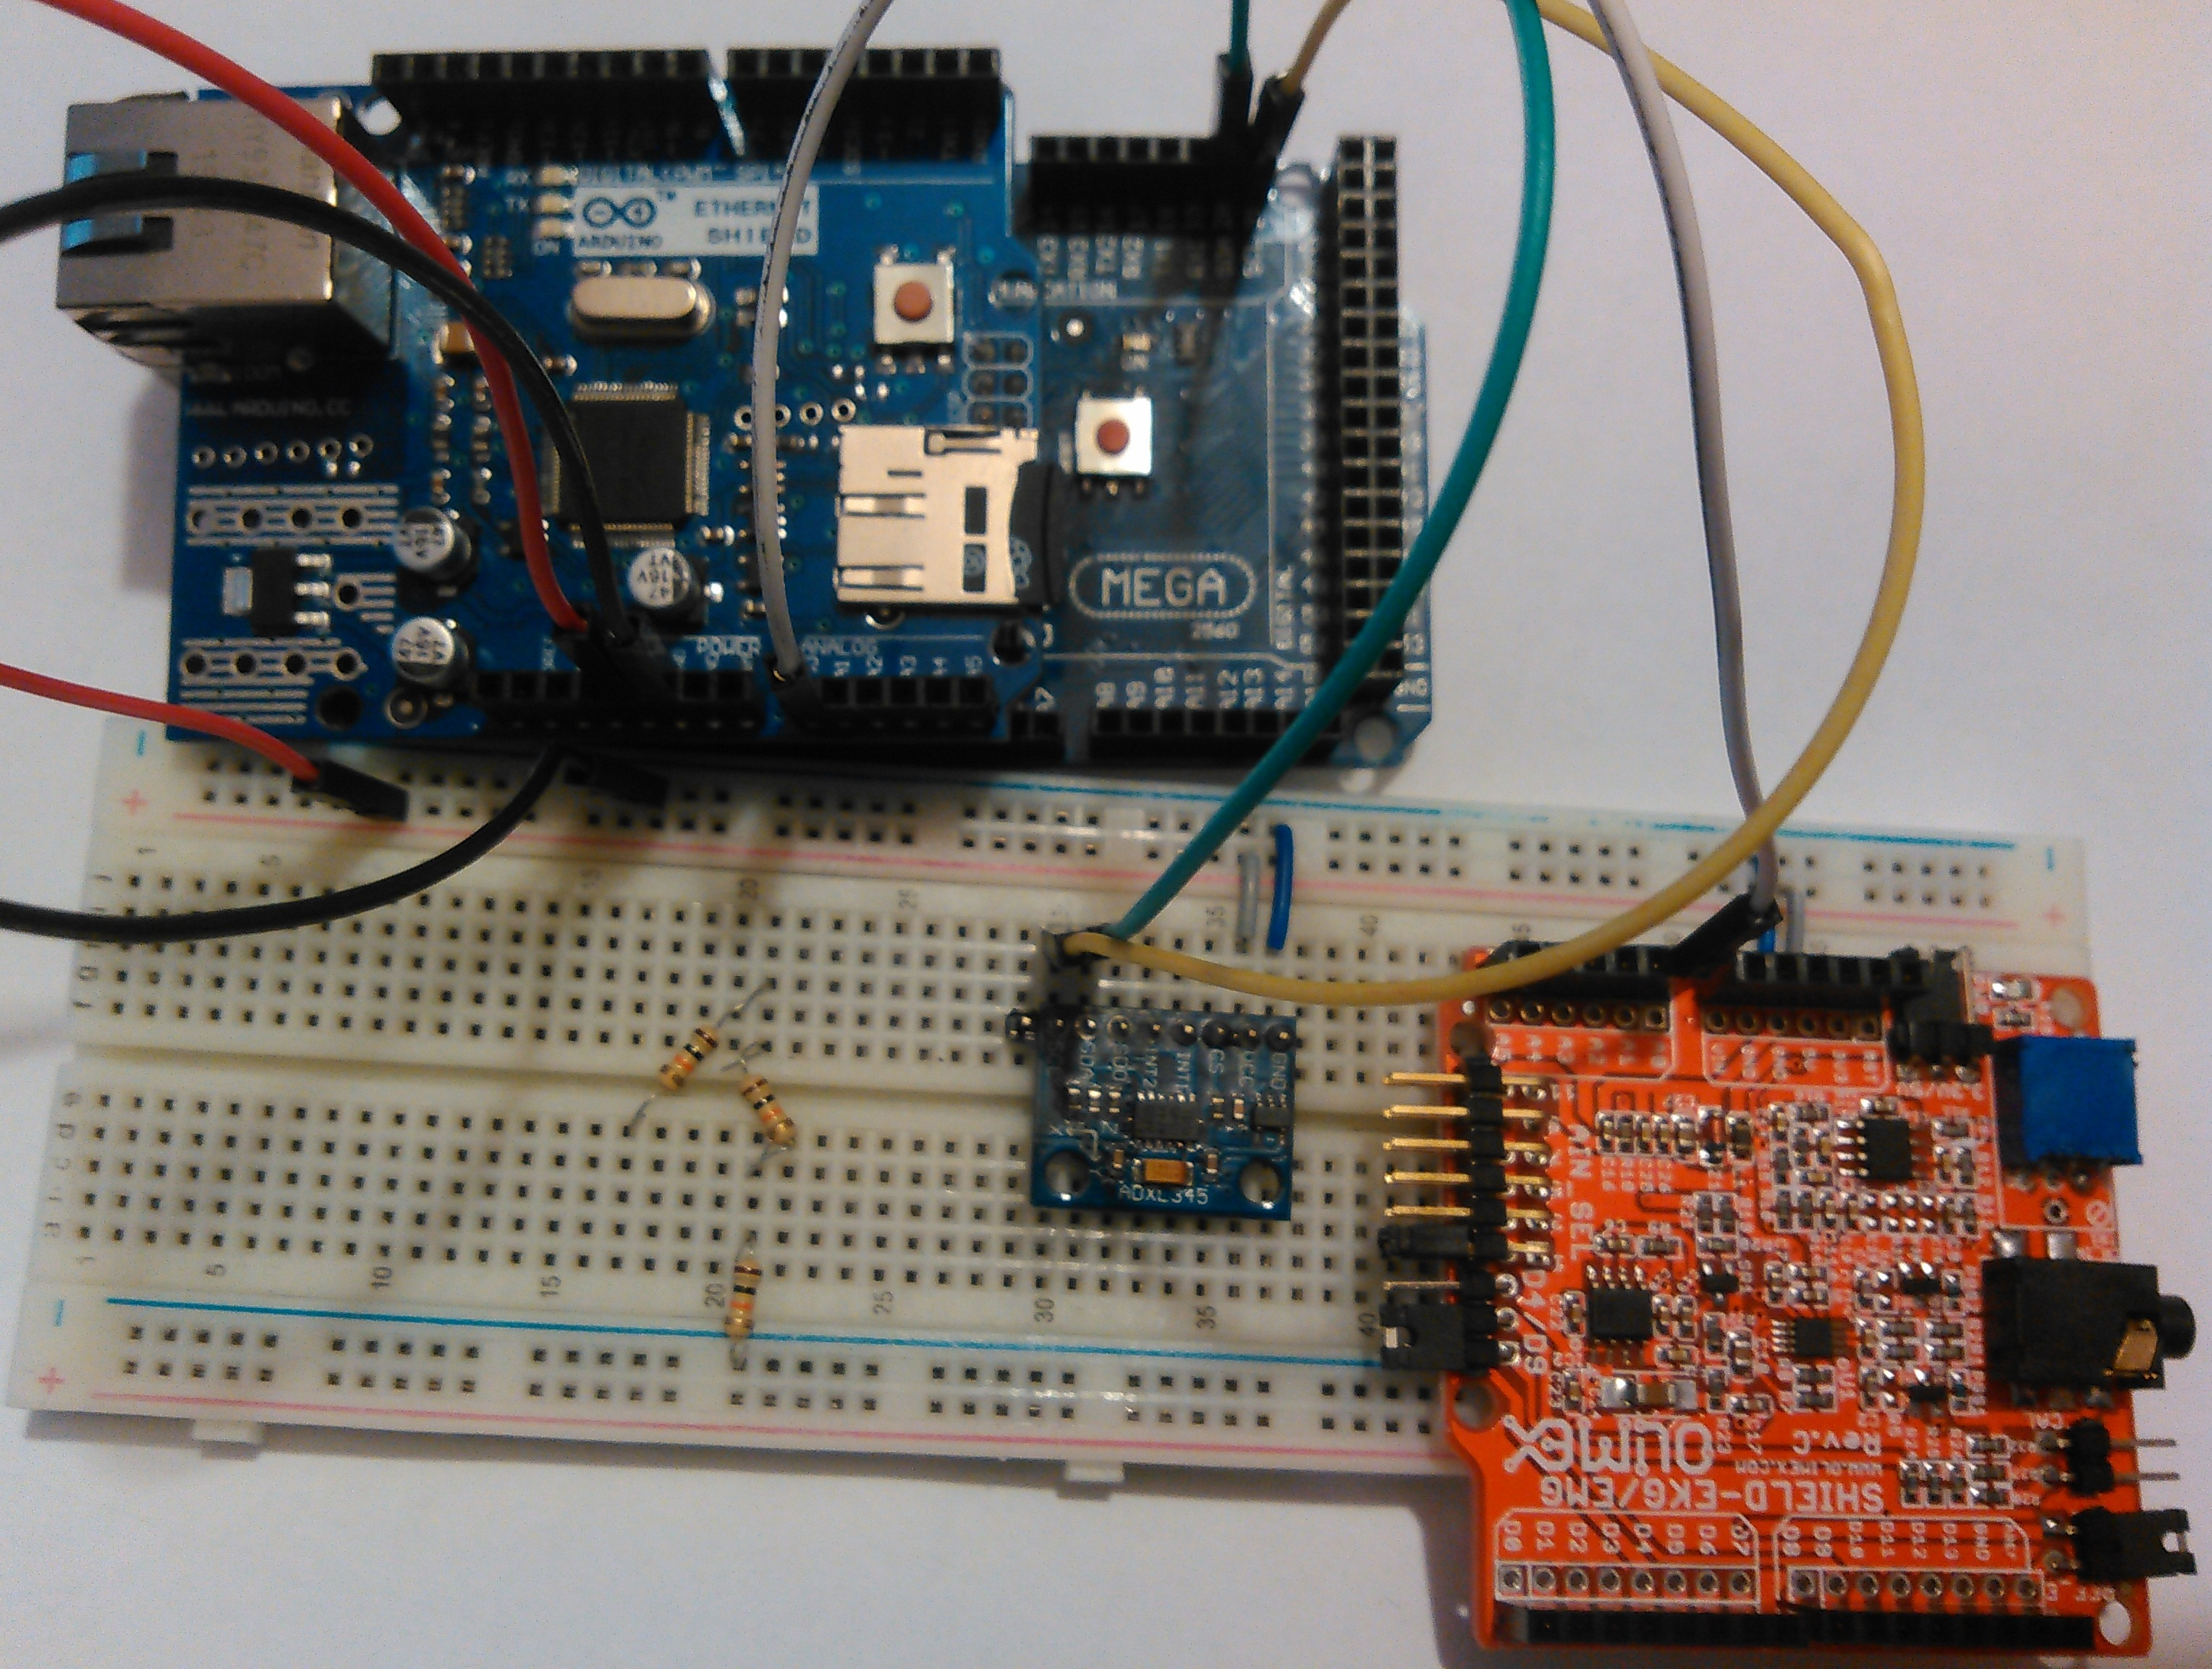
\includegraphics[width=0.8\textwidth]{29}
  	\end{center}
  	\caption{Wearable device design}
	\label{fig:28}
\end{figure}
\subsection{Proposed design}
Figure~\ref{fig:12} on page~\pageref{fig:12} shows the detailed flow chart of the project.
\begin{figure}[h]
  	\begin{center}
    	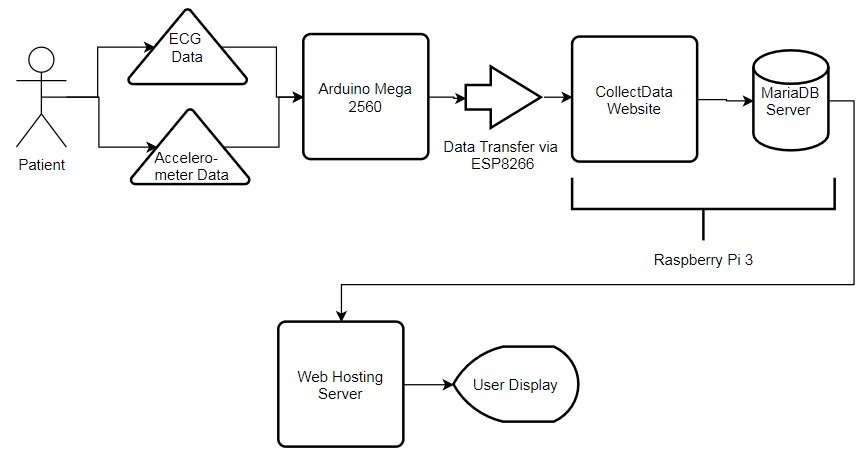
\includegraphics[width=1\textwidth]{12}
  	\end{center}
  	\caption{Project flowchart}
	\label{fig:12}
\end{figure}
In total 4 programming languages were used:
\begin{itemize}
\item \textbf{C,}
\item \textbf{Hypertext Preprocessor (PHP),}
\item \textbf{Structured Query Language (SQL),}
\item \textbf{C Sharp (C\#).}
\end{itemize}
And 3 different communication protocols:
\begin{itemize}
\item \textbf{Inter-Integrated Circuit (I$^2$C),}
\item \textbf{Hypertext Transfer Protocol (HTTP),}
\item \textbf{Secure Shell (SSH).}
\end{itemize}
Due to the complexity of the project, and many stages of data transfer, each written in a different programming language, it will be easier to further sub categorise the project into:
\begin{itemize}
\item[1] \textbf{The wearable device design,}
\item[2] \textbf{Server design,}
\item[3] \textbf{Displaying data.}
\end{itemize}
\subsubsection{Wearable device design}
The wearable device consists of: a breadboard, two sensor modules, a micro-controller board and a Ethernet shield. The two sensor modules used were: 
\begin{itemize}
\item[a] Olimex SHIELD-EKG-EMG see figure~\ref{fig:14} on page~\pageref{fig:14},
\item[b] Analog Devices ADXL 345 see figure~\ref{fig:33} on page~\pageref{fig:33}.
\end{itemize}
\begin{figure}
	\begin{center}
		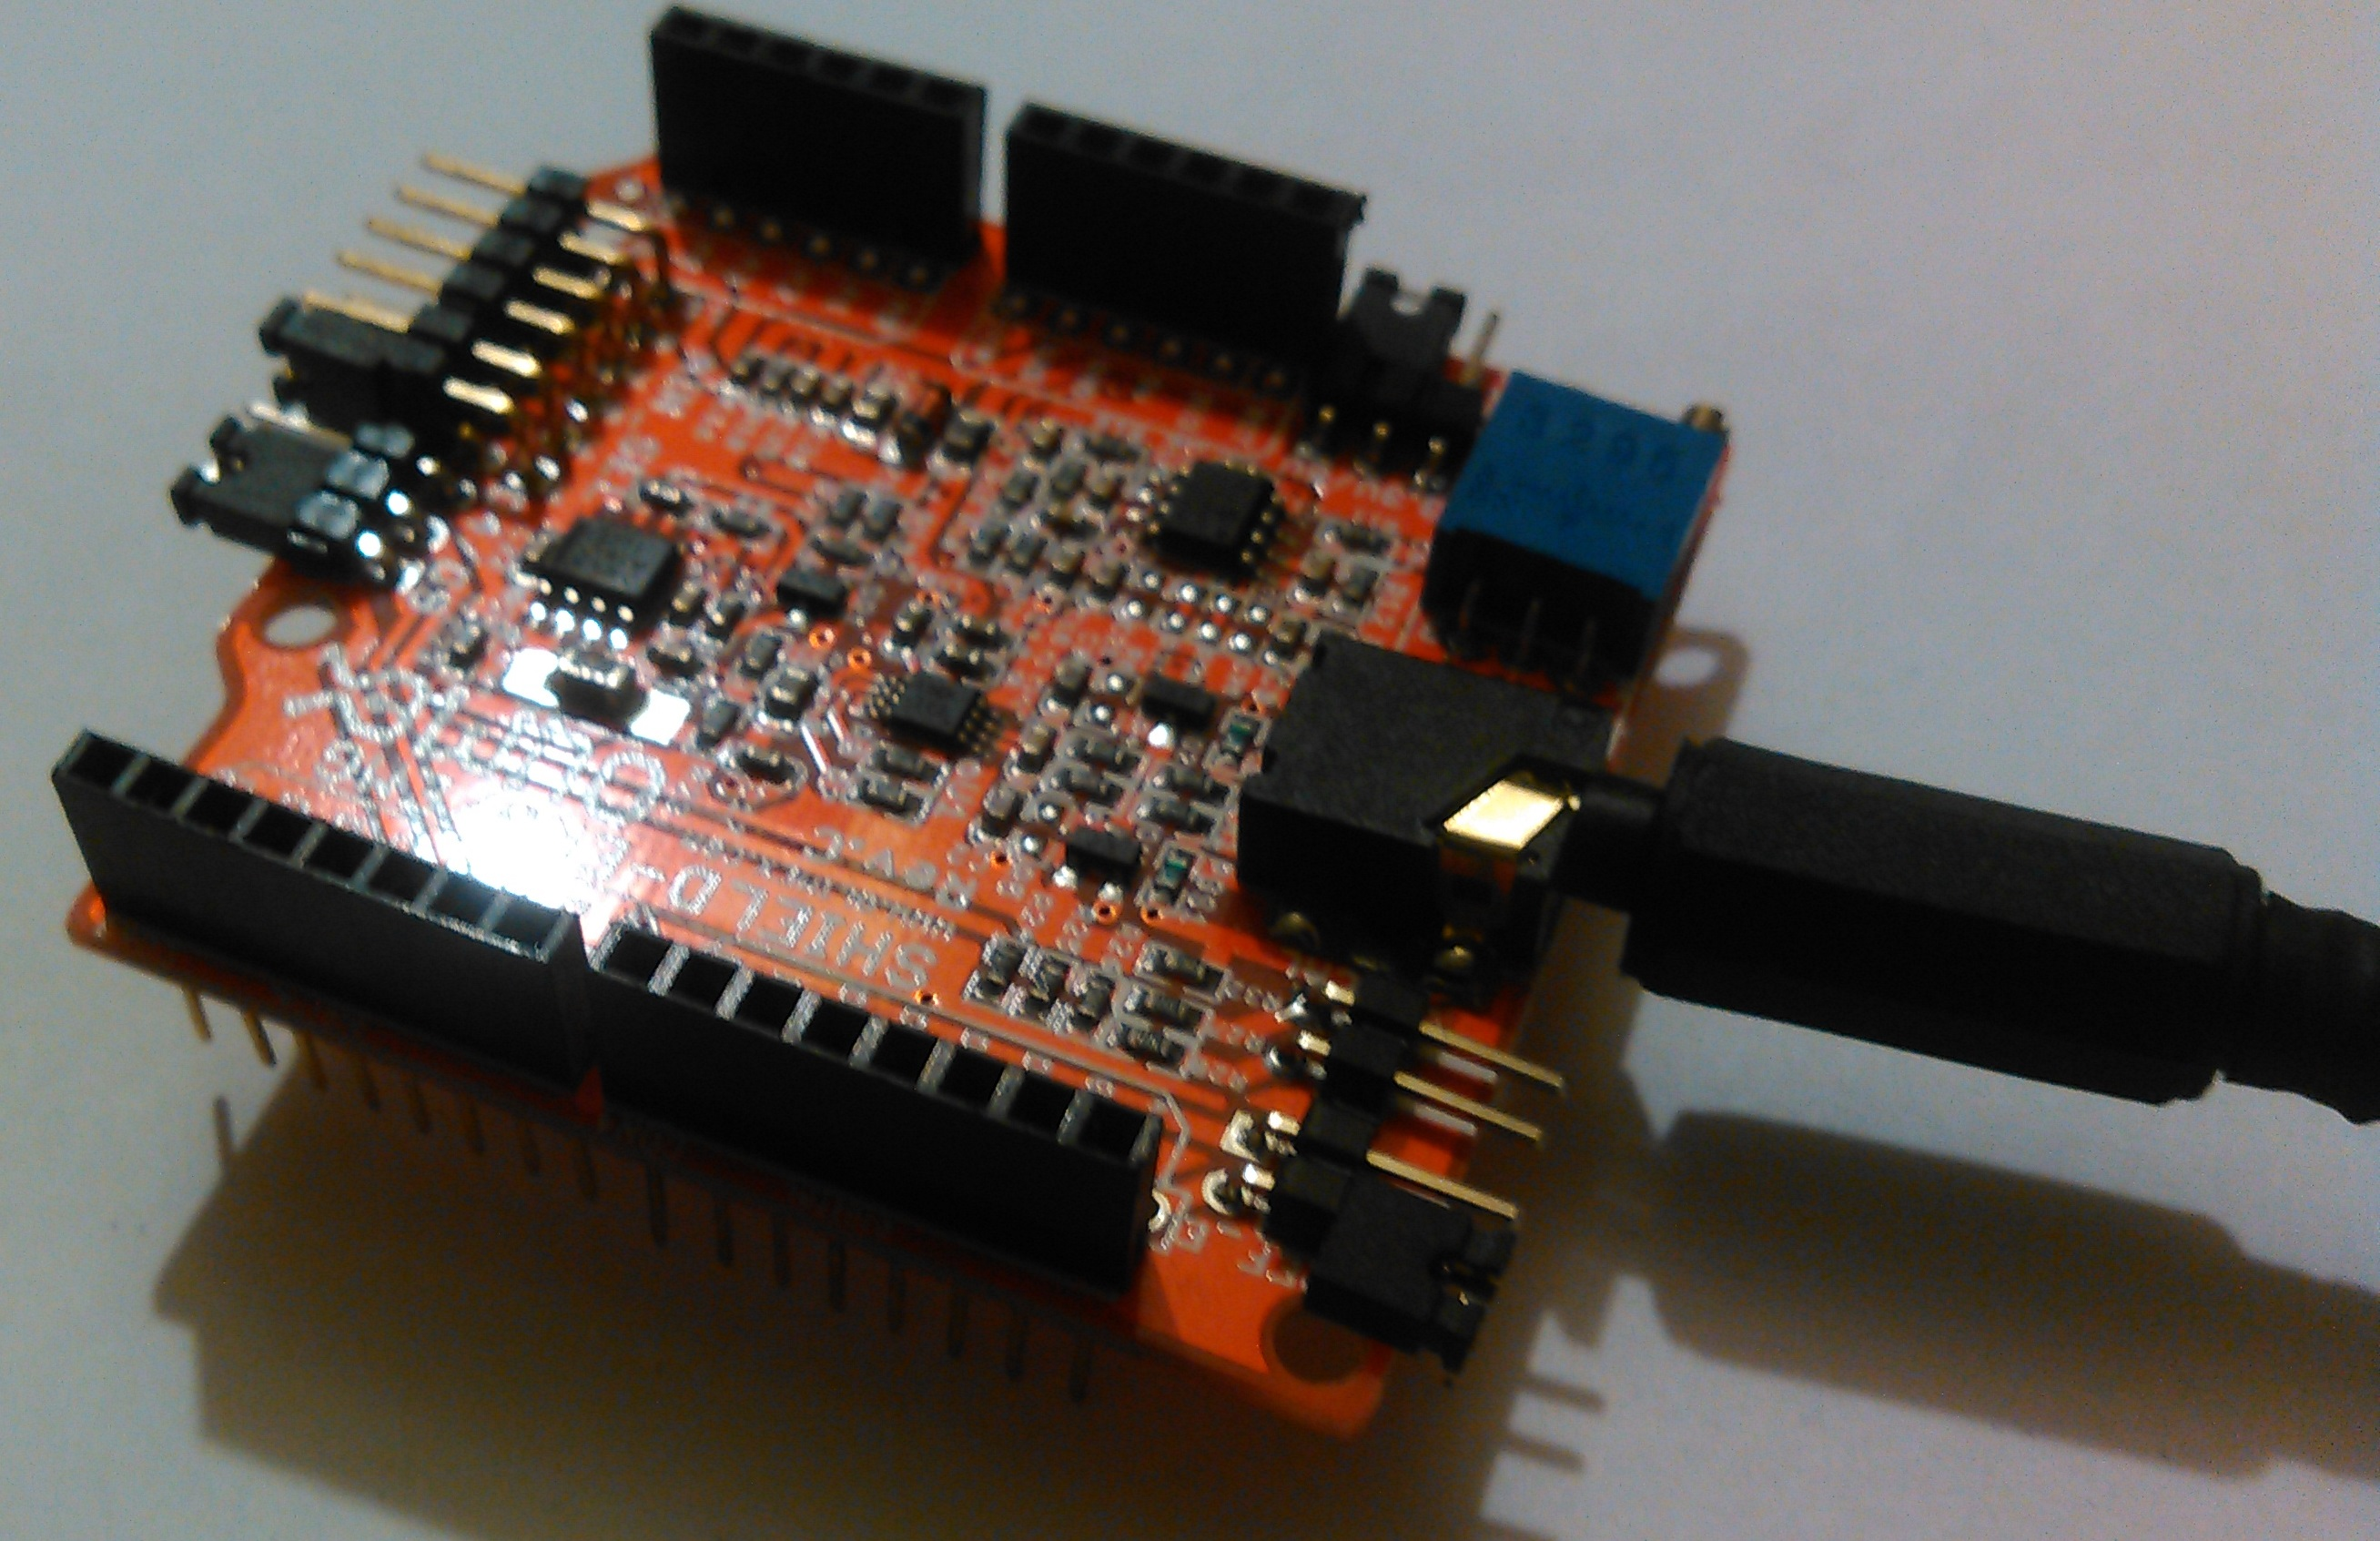
\includegraphics[width=0.8\textwidth]{13}
	\end{center}
    \caption{SHIELD-EKG-EMG}
	\label{fig:14}
\end{figure}
\begin{figure}
	\begin{center}
		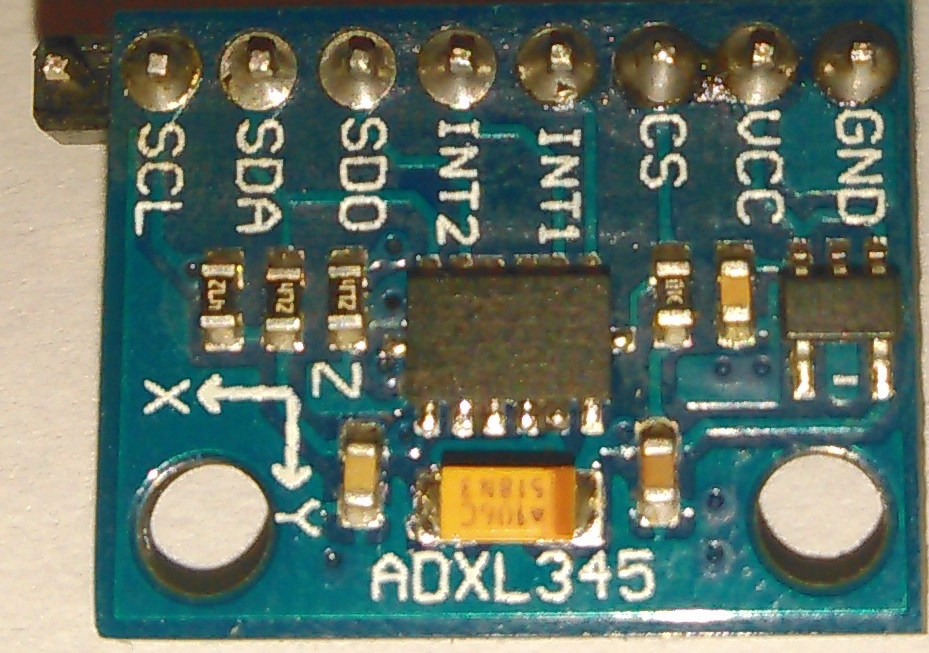
\includegraphics[width=0.8\textwidth]{14}
	\end{center}
    \caption{ADXL345}
	\label{fig:33}
\end{figure}
Arduino MEGA 2560 was used as the micro-controller board, the internet communication was done via Arduino Ethernet Shield, See figure~\ref{fig:16}, \ref{fig:34} on page~\pageref{fig:16} for the Arduino boards used.
\begin{figure}
	\begin{center}
		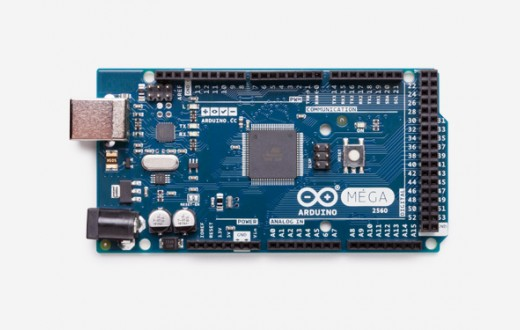
\includegraphics[width=0.8\textwidth]{15}
	\end{center}
    \caption{Arduino MEGA 2560 \cite{Arduino}}
	\label{fig:16}
\end{figure}
\begin{figure}
	\begin{center}
		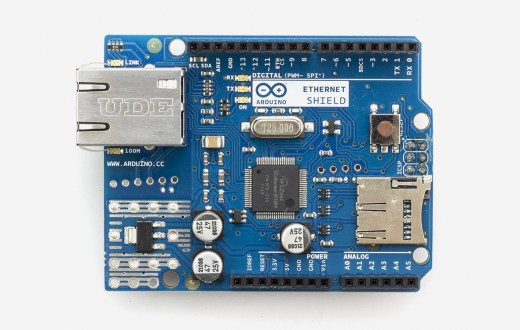
\includegraphics[width=0.8\textwidth]{16}
	\end{center}
    \caption{Arduino Ethernet Shield \cite{Arduino}}
	\label{fig:34}
\end{figure}
\subsubsection{Server design}
Raspberry pi 3 was used as the server. First apache2 server had to be installed to host web pages, then php7 and MaridDB to handle the data. For detailed installation notes see the installation guide. Figure~\ref{fig:17} on page~\pageref{fig:17} shows what Raspberry Pi 3 looks like.
\begin{figure}[h]
  	\begin{center}
    	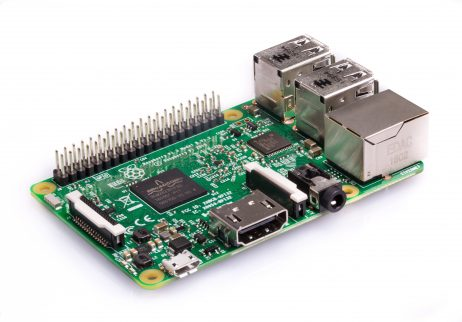
\includegraphics[width=0.8\textwidth]{17}
  	\end{center}
  	\caption{Raspberry Pi 3 \cite{Raspberry Pi}}
	\label{fig:17}
\end{figure}
\subsubsection{Displaying the data}
A Model-View-Controller (MVC) ASP.NET web application was used to display the data. Figure~\ref{fig:18} on page~\pageref{fig:18} shows what the web application looks like.
\begin{figure}[h]
  	\begin{center}
    	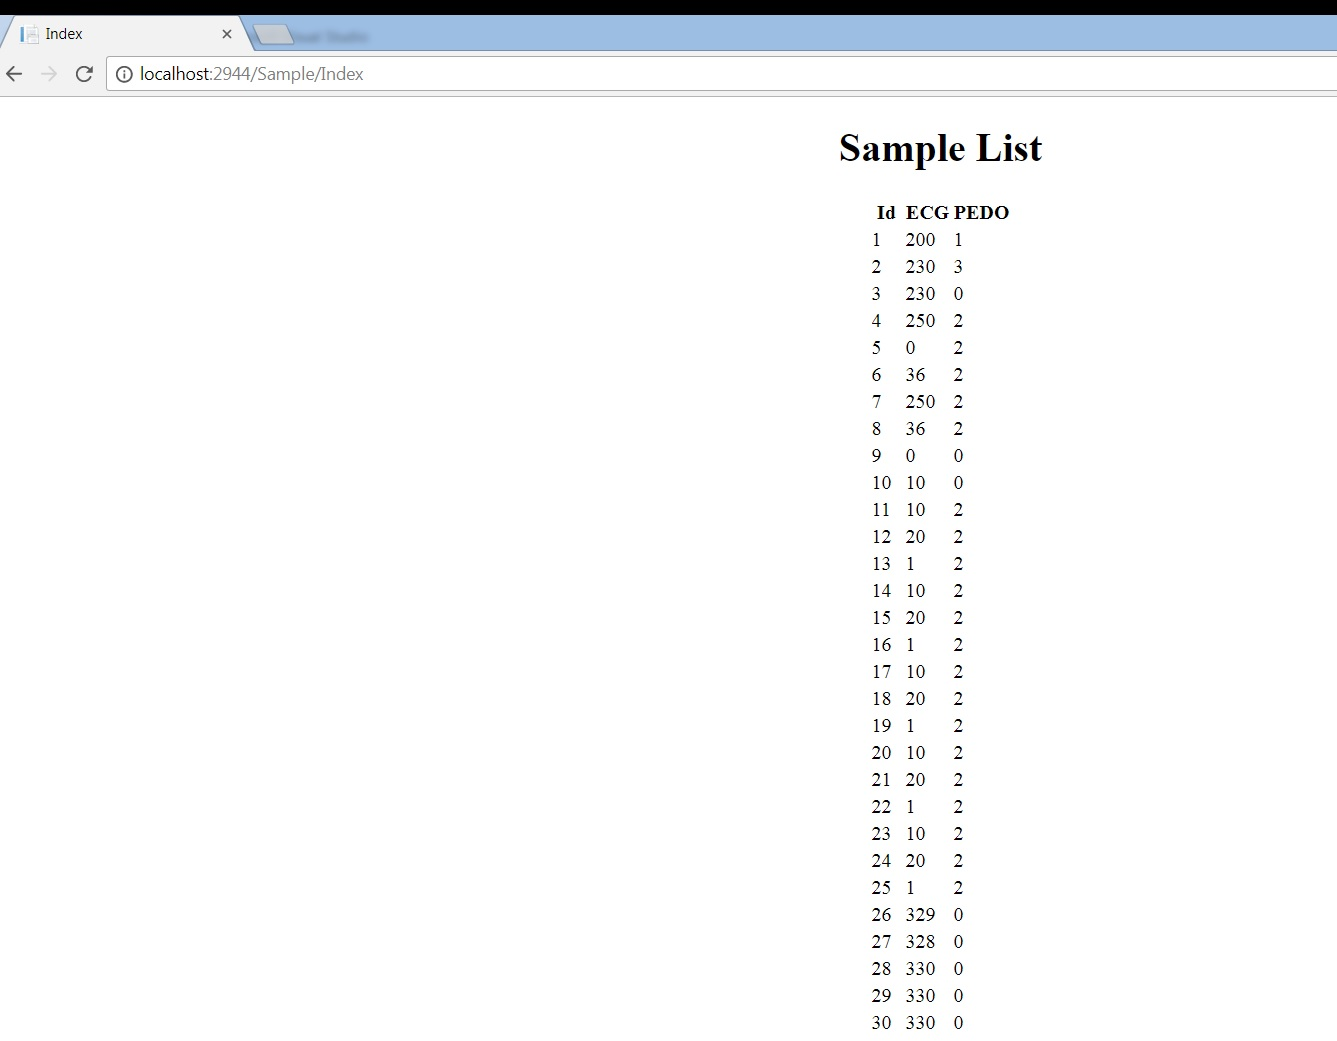
\includegraphics[width=0.8\textwidth]{18}
  	\end{center}
  	\caption{Web application}
	\label{fig:18}
\end{figure}
\newpage
\section{Internal specification}
The whole project can be categorised with respect to the programming language used. There for there will be 4 subsections: C, PHP, SQL and C\# respectively. with the exception of SQL, all the files containing the discussed code can be found in the '/Code/' directory provided the root directory is the project CD/DVD drive, this will always be the case when directory navigation is mentioned unless specified otherwise.
\subsection{C}
C is the code that is executed by the Arduino MEGA 2560 micro-controller. It measures or requests measurements from the modules attached, then it processes the data and finally sends the data to the server via the Ethernet module. The SendData.ino located in the '/Code/Arduino/SendData/' directory contains all the code that will be discussed in this subsection. This part of the project also requires cable connections to be made between the micro-controller and modules. GND to GND and 5V to VCC have to be made on all boards with the exception of the ESP8266 module witch can only take 3.3V. Table~1 on page~\pageref{tab:1} shows how all other connections are to be made.
\begin{table}[h]
	\begin{center}
	\begin{tabular}{|p{5cm}|p{5cm}|}
		\hline
		Pin number on Arduino MEGA board & Pin number on 			module\\
		\hline
		A0 & A0 on the Olimex EKG-SHIELD\\
		\hline
		SDA 20 & SDA 7 on ADXL 345\\
		\hline
		SCL 21 & SCL 8 on ADXL 345\\
		\hline
		\multicolumn{2}{ |c| }{If connecting the Arduino 			Ethernet module} \\
		\hline
		RX0 & RX0\\
		\hline
		IOREF & IOREF\\
		\hline
		\multicolumn{2}{ |c| }{If connecting the ESP8266 			module}\\
		\hline
		RX0 & RX\\
		\hline
		TX0 & TX\\
		\hline
		GND & GND\\
		\hline
		3.3V & 3.3V\\
		\hline		
		GND & IO0\\
		\hline
		3.3V & EN\\
		\hline
	\end{tabular}
	\end{center}
	\label{tab:1}
	\caption{Table of connections}
\end{table}
\subsubsection{Collecting ECG data}
Collecting ECG data is very straightforward because all that is needed is a analogue to digital conversion of the A0 pin on the Olimex shield. But the sampling rate has to be consistent there for a timer interrupt has to be used to achieve this. Arduino MEGA 2560 has 6 built in timers, timer0 to timer5. Timer5 has been configured as this timer is not used by the delay() function and the Wire library as well as the PWM outputs are located at pins 44, 45 and 46.  A sampling rate of 200Hz will be used as it is the smallest sampling rate at witch the ECG signal can still analysed. Using the function:
\begin{equation}
Timer speed(Hz)= \frac{Arduino clock speed (16MHz)}{prescaler*(compare match register+1)}
\end{equation}
By rearranging the equation and using a 64 prescaler, compare match register value can be found as it is needed to set the correct frequency:
\begin{equation}
compare match register=\left(\frac{16000000}{64*200}\right)-1
\end{equation}
The compare match register value is 1249, it is possible to set this value as greater than 256 because timer5 is a 16bit timer therefore the maximum register value is 65536.
\subsubsection{Collecting Pedometer data}
The Pedometer data first has to be collected. First the ADXL345 accelerometer data has to be pulled up. This is done using I$^2$C serial communication. Serial Peripheral Interface (SPI) could also be used, but it requires a greater number of connections (4 in case of SPI and only 2 in case of I$^2$C). For this protocol the sensor address and the data registers address have to be known. In this case the sensor address is 0x53 and the data registers addresses are 0x32 to 0x37, where 0x32 (DATAX0) and 0x33 (DATAX1) are the data registers addresses for the X-Axis. Both registers contain 8 bits of data that have to be combined for a 16 bit X-Axis measurement. The DATAX1 register contains the most significant bits (MSB) of the 16 bit number. The same operation needs to be done to the Y and Z axis, 0x34 (DATAY0) and 0x35 (DATAY1) are both are the Y-Axis register addresses with the DATAY1 containing the MSB, 0x36 (DATAZ0) and 0x37 (DATAZ1) are both are the Z-Axis register addresses with the DATAZ1 containing the MSB.\\
These values are then squared and summed. The sum is later compared to a threshold value and if the sum is greater than the threshold value then a step-counter is incremented and returned.
\subsubsection{Sending data}
Originally the wearable device was intended to be wireless. But due to electrical problems the ESP8266 Wi-Fi module could not be used. This was because Arduino MEGA 2560 can supply a maximum current of 50mA on the 3.3V pin and the ESP8266 wifi module at peak power consumption when transferring data over Wi-Fi network, requires 400mA. And therefore the module reset when insufficient power to the module was provided. Also the breadboard used to power all the devices with an inbuilt, 3.3V stabilizer could not be used to power the ESP8266 Wi-Fi module as the 3.3V ground and the 5V ground of the breadboard power supply had a voltage difference of 1.5V. This would make it impossible for the ESP8266 Wi-Fi module to communicate with Arduino MEGA 2560 as they would not share a common ground. And due to time constraint buying and waiting for voltage stabiliser was not an option. Nevertheless both the Ethernet shield and the ESP8266 Wi-Fi shield code files are included in the '/Code/Arduino/Transferring Data/' directory. But ultimately the Ethernet shield code was used in the SendData.ino file. To send the data first the IP address of the Raspberry Pi 3 server has to be known. In this case it is 192.168.0.38. After a successfully connection to the server as a client the POST request can be sent. 
\begin{verbatim}
POST /collectdata.php HTTP/1.1
Host: 192.168.0.38
Accept: */*
Content-Length: 32
Content-Type: application/x-www-form-urlencoded

ecg=ecgString&pedo=NumberOfSteps
\end{verbatim}
First the request method is specified in this case POST, then the file is specified and the HTTP protocol version. Another key part of the POST request is the Content-Type specifier as well as Content-Length. And finally the parameter name and values are specified, in case of more than one parameter each successive parameter is added after the \& sign. The post method was used as it has no data length restraint compared to a GET request.
\subsection{PHP}
The $collectdata.php$ file contains the PHP code that is executed every time it is requested, the file can be found in the '/Code/' directory. First two values ecgString and pedo are created and inherit values from their POST equivalent. Because ECG data is sent as a long string where each value is separated with a "," from the next one the built in $expolde()$ function is used to separate the values and inserts the into a$ecgArray$. Next a $mysqli\_connect$ link is created that will grant access to the database. If link execution is successfully, data is inserted into an existing table "patient1". After the data has been inserted into the table the connection is closed.
\subsection{SQL}
First, two new users have to be created. One that will have access to the database from the php file and the other that will have external access from the MVC web application. This is done using: 
\begin{verbatim}
create user 'collect'@'localhost' identified by 'data';
create user 'proj'@'localhost' identified by 'mnp';
\end{verbatim} 
Next the database that will store the ECG and Pedometer data is created, this is done using the querry: 
\begin{verbatim}
create database ecgpedodata;
\end{verbatim}
After the database has been created a table has to be created to store data:
\begin{verbatim}
USE ecgpedodata;
CREATE TABLE patient1 (id MEDIUMINT NOT NULL AUTO_INCREMENT, ecg SMALLINT 
NOT NULL, pedo TINYINT NOT NULL);
\end{verbatim}
All that is left is to grant access to the crated users to ecgpedadata database.
\begin{verbatim}
GRANT ALL PRIVILEGES ON ecgpedodata.* TO 'collect'
@'localhost' IDENTIFIED BY 'data';
GRANT ALL PRIVILEGES ON ecgpedodata.* TO 'proj'
@'192.168.0.%' IDENTIFIED BY 'mnp';
\end{verbatim}
The first user only needs to access the database on local host , but the website needs to be able to access the database remotely therefore a "\%" which will allow the proj user to log into the database from any Internet Protocol (IP) dress on the local network.
\subsection{C\#}
Because the Raspberry Pi 3 server is a MySQL server and not a SQL server a MySQL.Data NuGet package has to be installed for the server to recognise the queries as show by figure \ref{fig:20}, \ref{fig:35} on page~\pageref{fig:20}, \pageref{fig:35}.
\begin{figure}[H]
	\begin{center}
		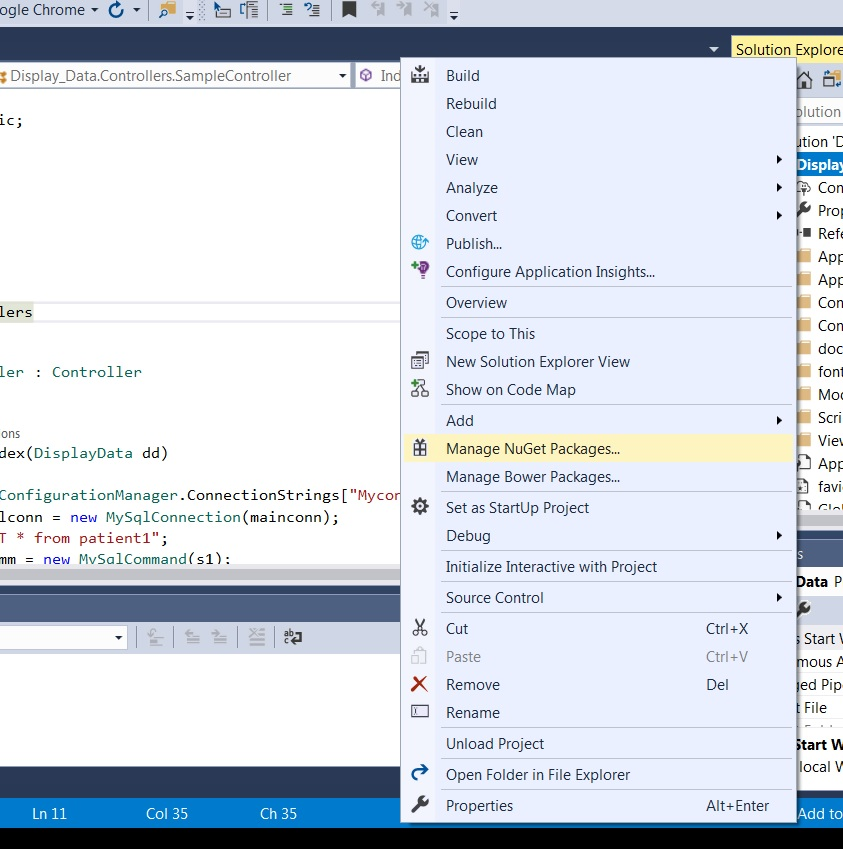
\includegraphics[width=0.8\textwidth]{19}
	\end{center}
    \caption{Manage NuGet packages option}
	\label{fig:20}
\end{figure}
\begin{figure}[H]
	\begin{center}
		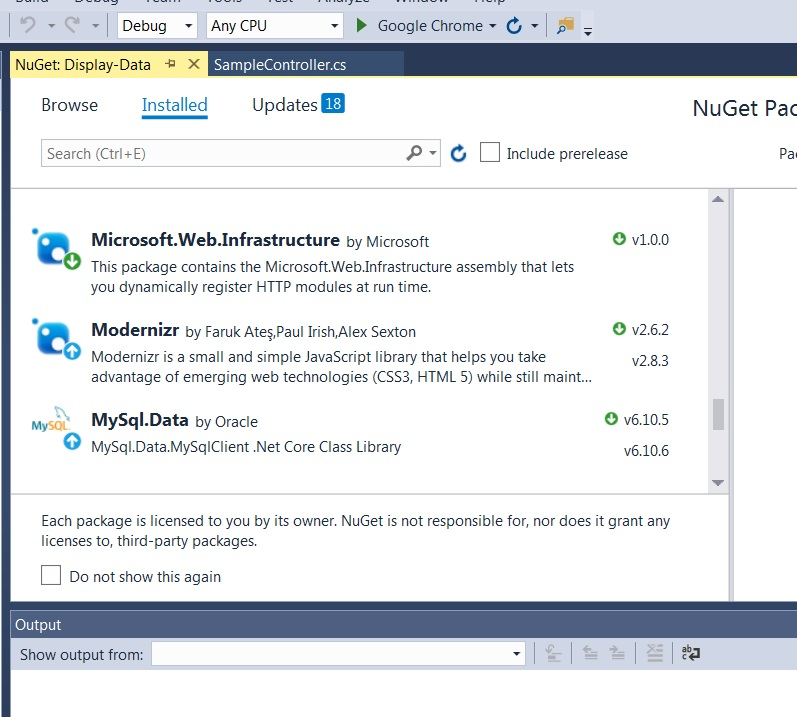
\includegraphics[width=0.8\textwidth]{20}
	\end{center}
    \caption{NuGet packages manager}
	\label{fig:35}
\end{figure}
A connection string has to be added to Web.config file that specifies the servers IP address the database and the user details.
\begin{verbatim}
<add name="Myconn" connectionString="Data Source=192.168.0.38;
port=3306; Initial Catalog=ecgpedodata;User Id=proj;password=mnp" />
\end{verbatim}
In the SampleController.cs using the directive MySql.Data.MySqlClient a connection to the Raspberry Pi server is established and data from ecgpedodata database, table patient1 is accessed. Which is then displayed as a table by Index.cshtml.
\newpage
\section{External specification}
For full Raspberry Pi installation and set-up see the Instalation.pdf file located in the '/Raport/' directory. To set up the wearable device, first the electrodes \ref{fig:22} on page~\pageref{fig:22}, have to be placed on the body of the patient, see figure \ref{fig:36} on page~\pageref{fig:36}. It is good practice to shave the hair under the electrode prior to application.
\begin{figure}[H]
	\begin{center}
		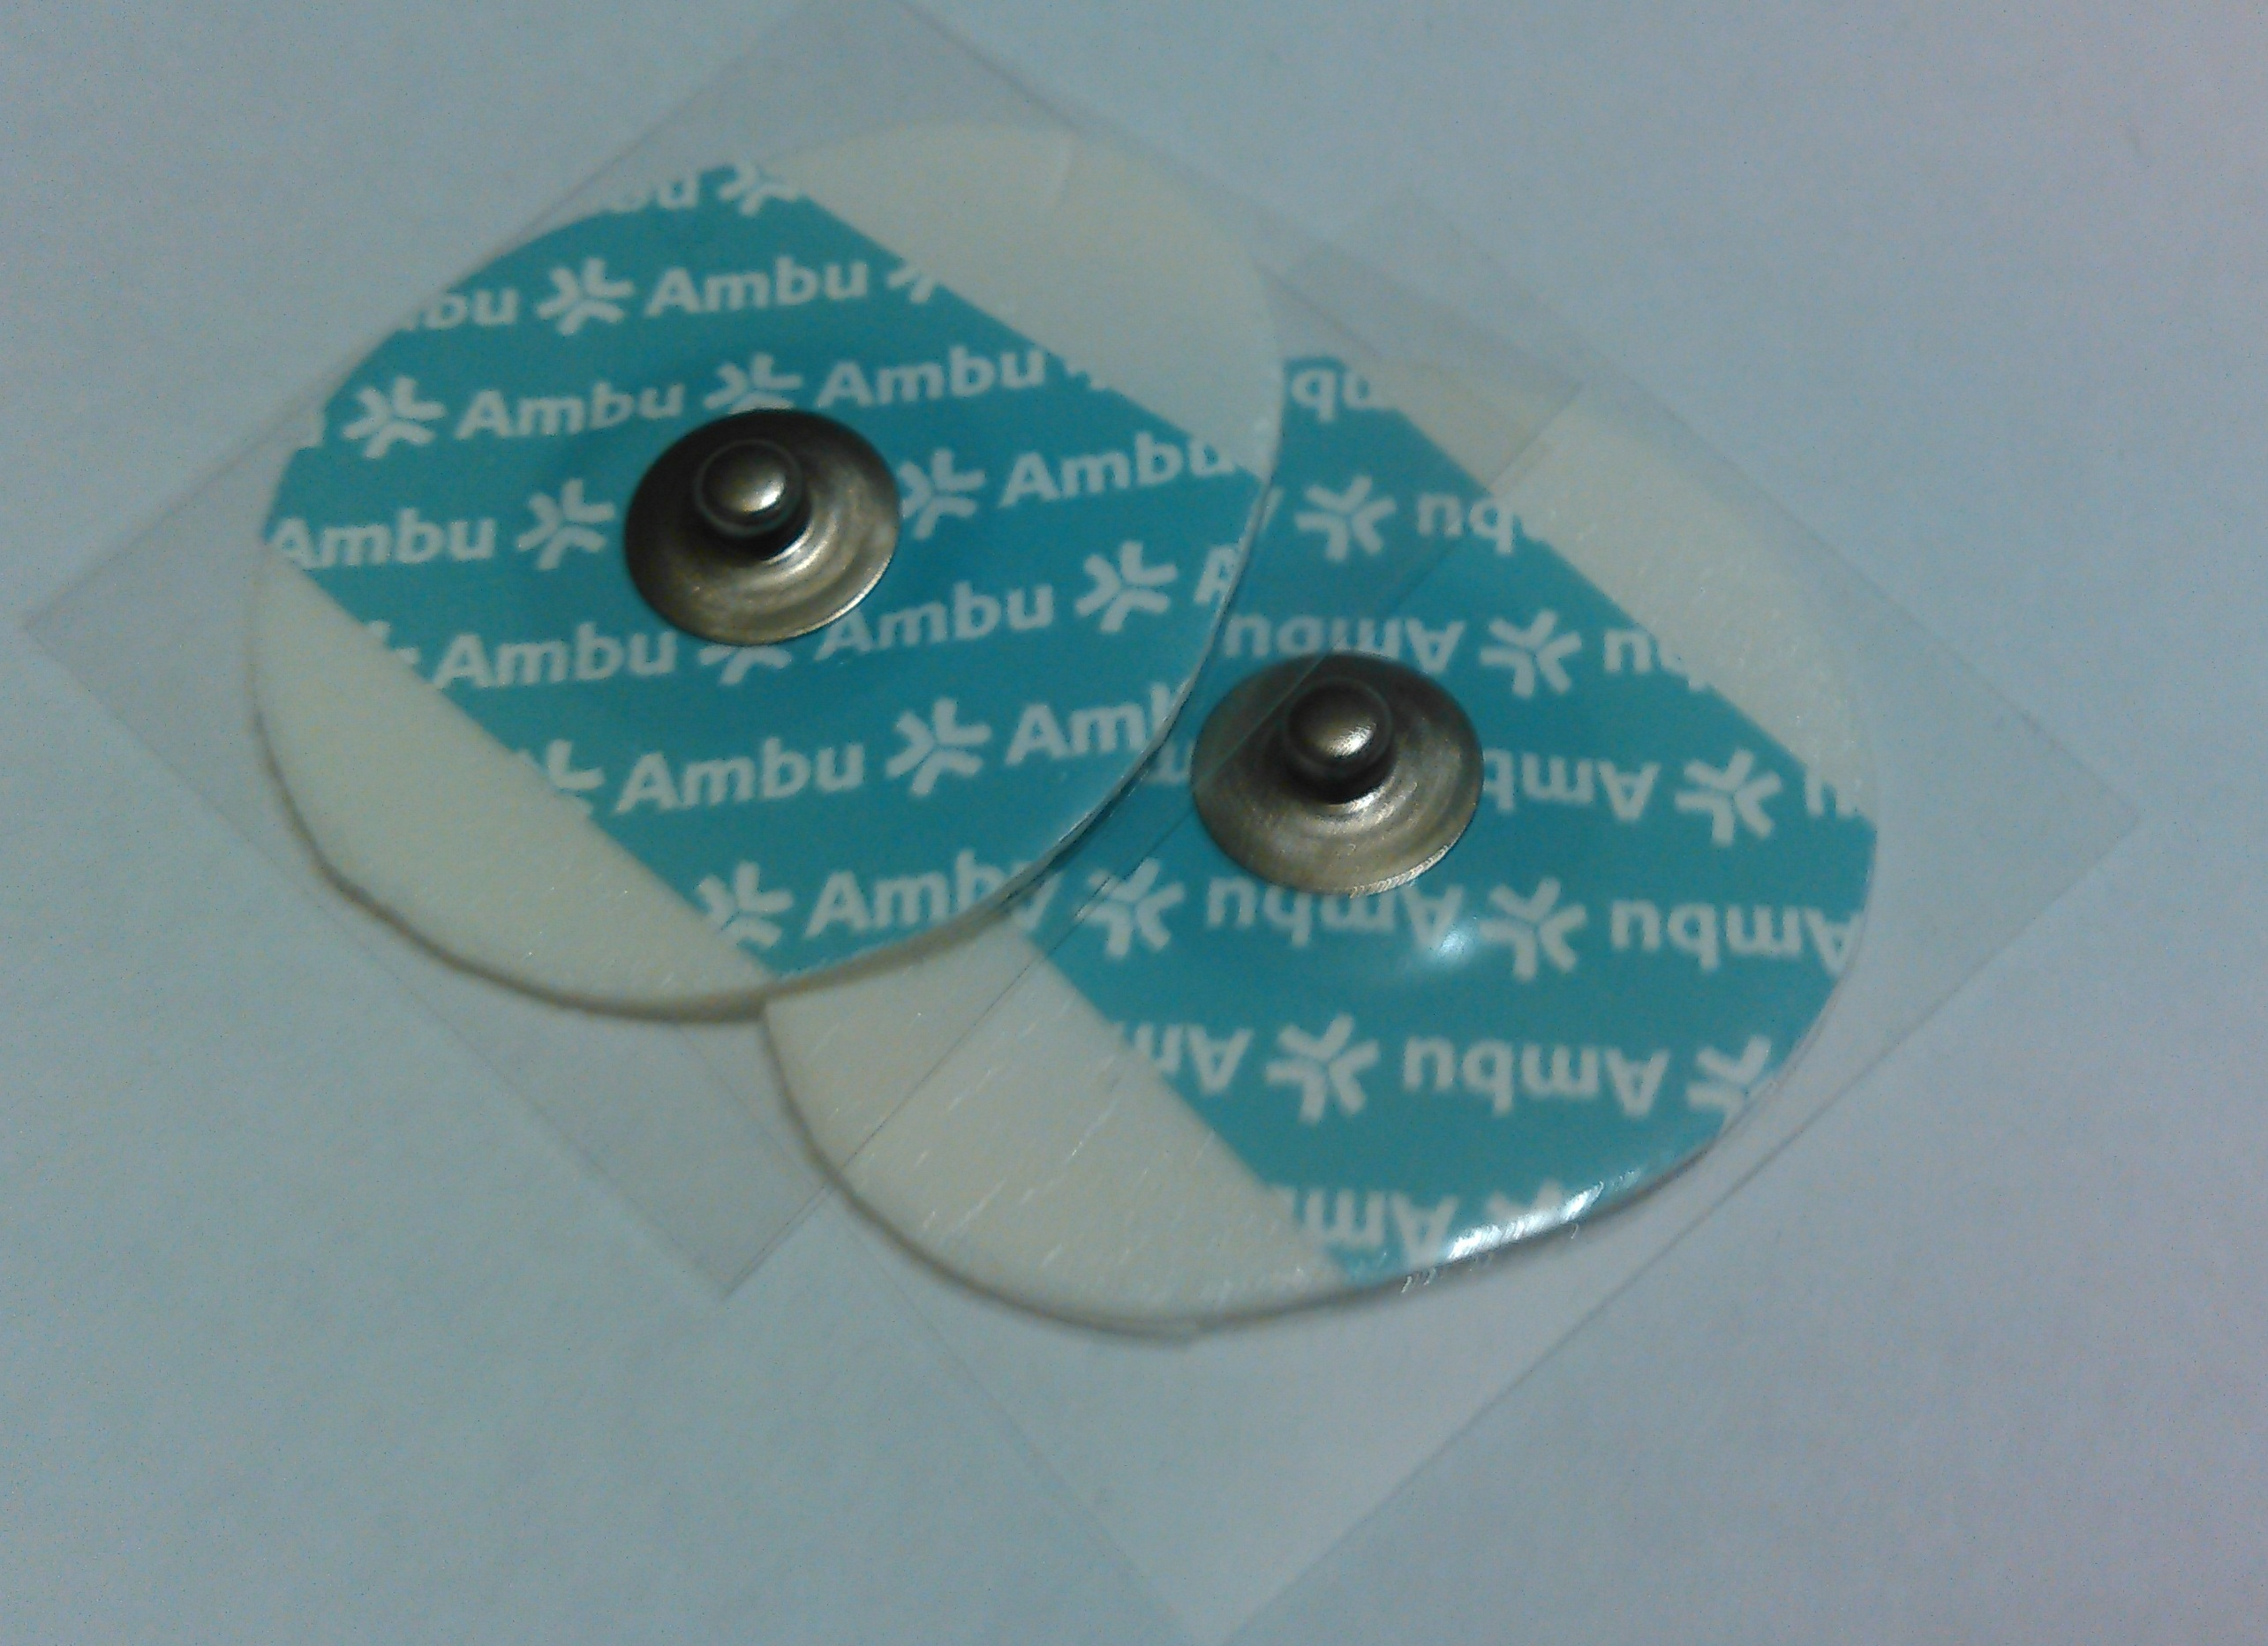
\includegraphics[width=0.8\textwidth]{21}
	\end{center}
    \caption{Electrodes}
	\label{fig:22}
\end{figure}
\begin{figure}[H]
	\begin{center}
		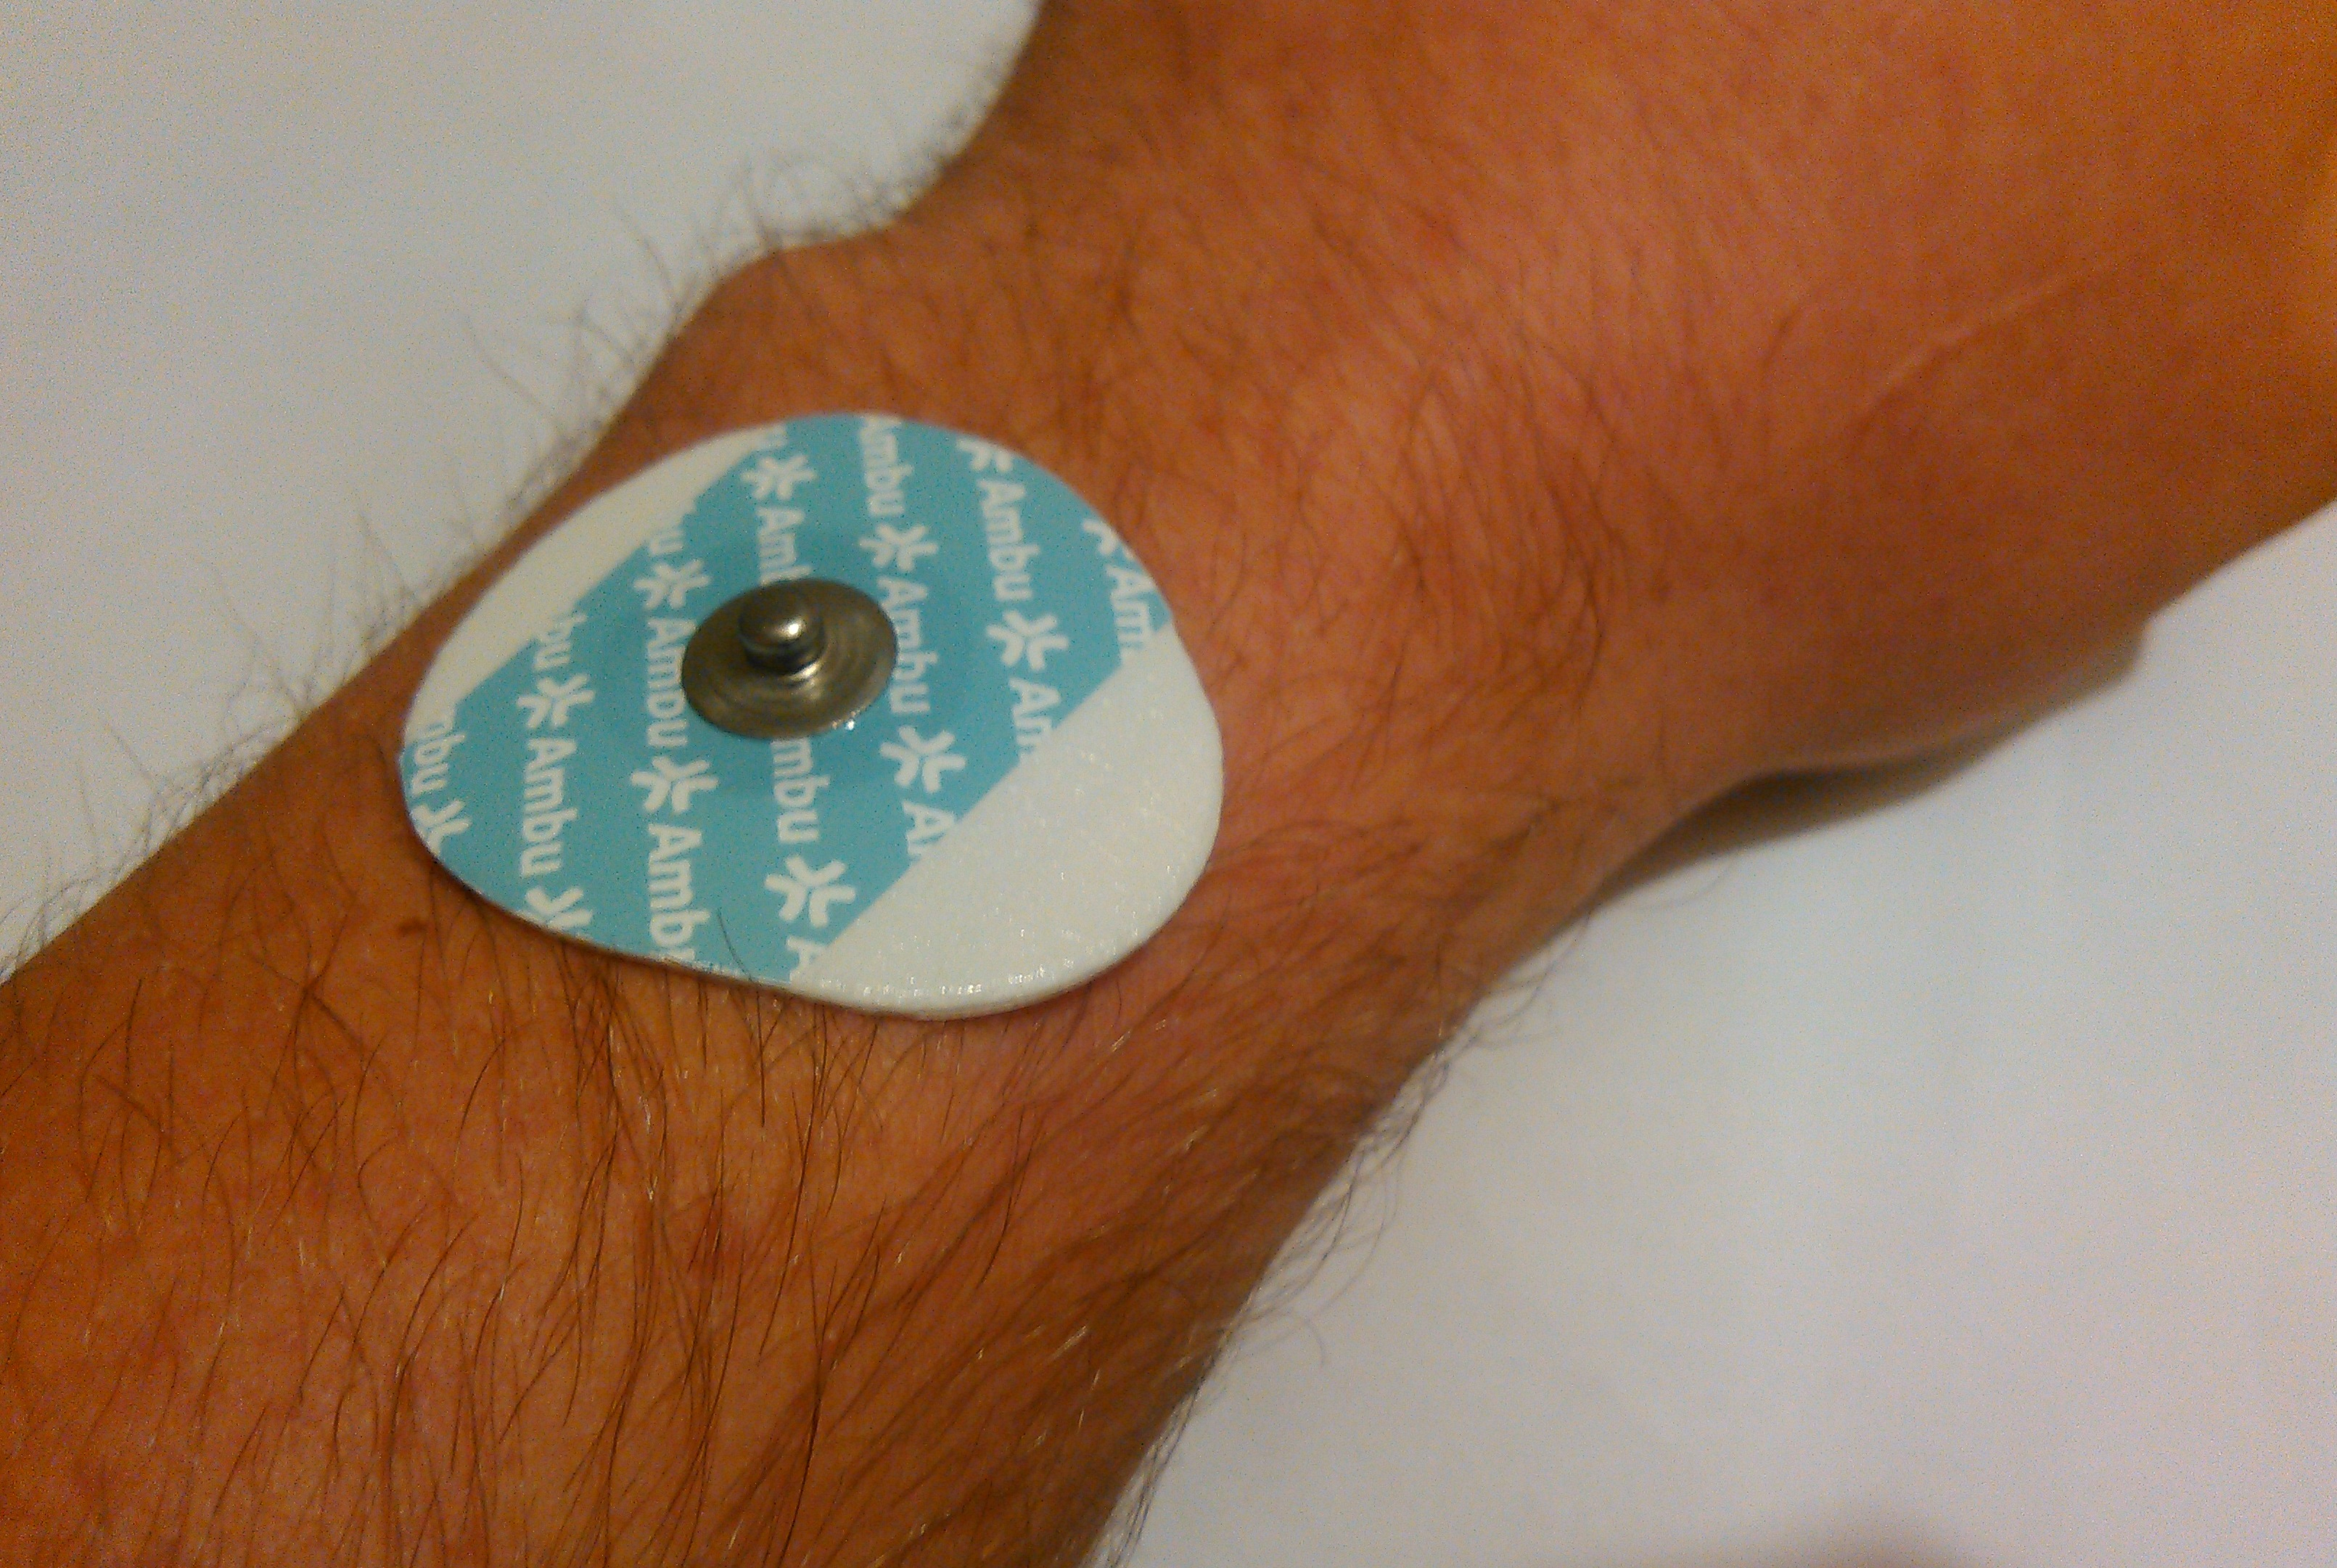
\includegraphics[width=0.8\textwidth]{22}
	\end{center}
    \caption{Electrode on the patient}
	\label{fig:36}
\end{figure}
Next attach the leads to the electrode and plug in the jack end of the cable to into Olimex SHIELD-EKG-EMG, it should be noted that red lead attaches to the right arm electrode, white lead attaches to the left arm electrode and the black lead attaches to the left ankle, see figure \ref{fig:25}, \ref{fig:37}, \ref{fig:38}. Figure~\ref{fig:14} on page~\pageref{fig:14} shows how the jack end of the leads plugs in to the Olimex SHIELD-EKG-EMG.
\begin{figure}[H]
	\begin{center}
		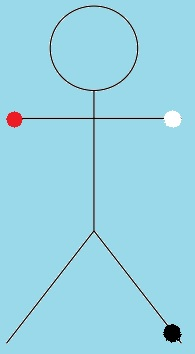
\includegraphics[width=0.3\textwidth]{23}
	\end{center}
    \caption{Lead colour placement}
	\label{fig:25}
\end{figure}
\begin{figure}[H]
	\begin{center}
		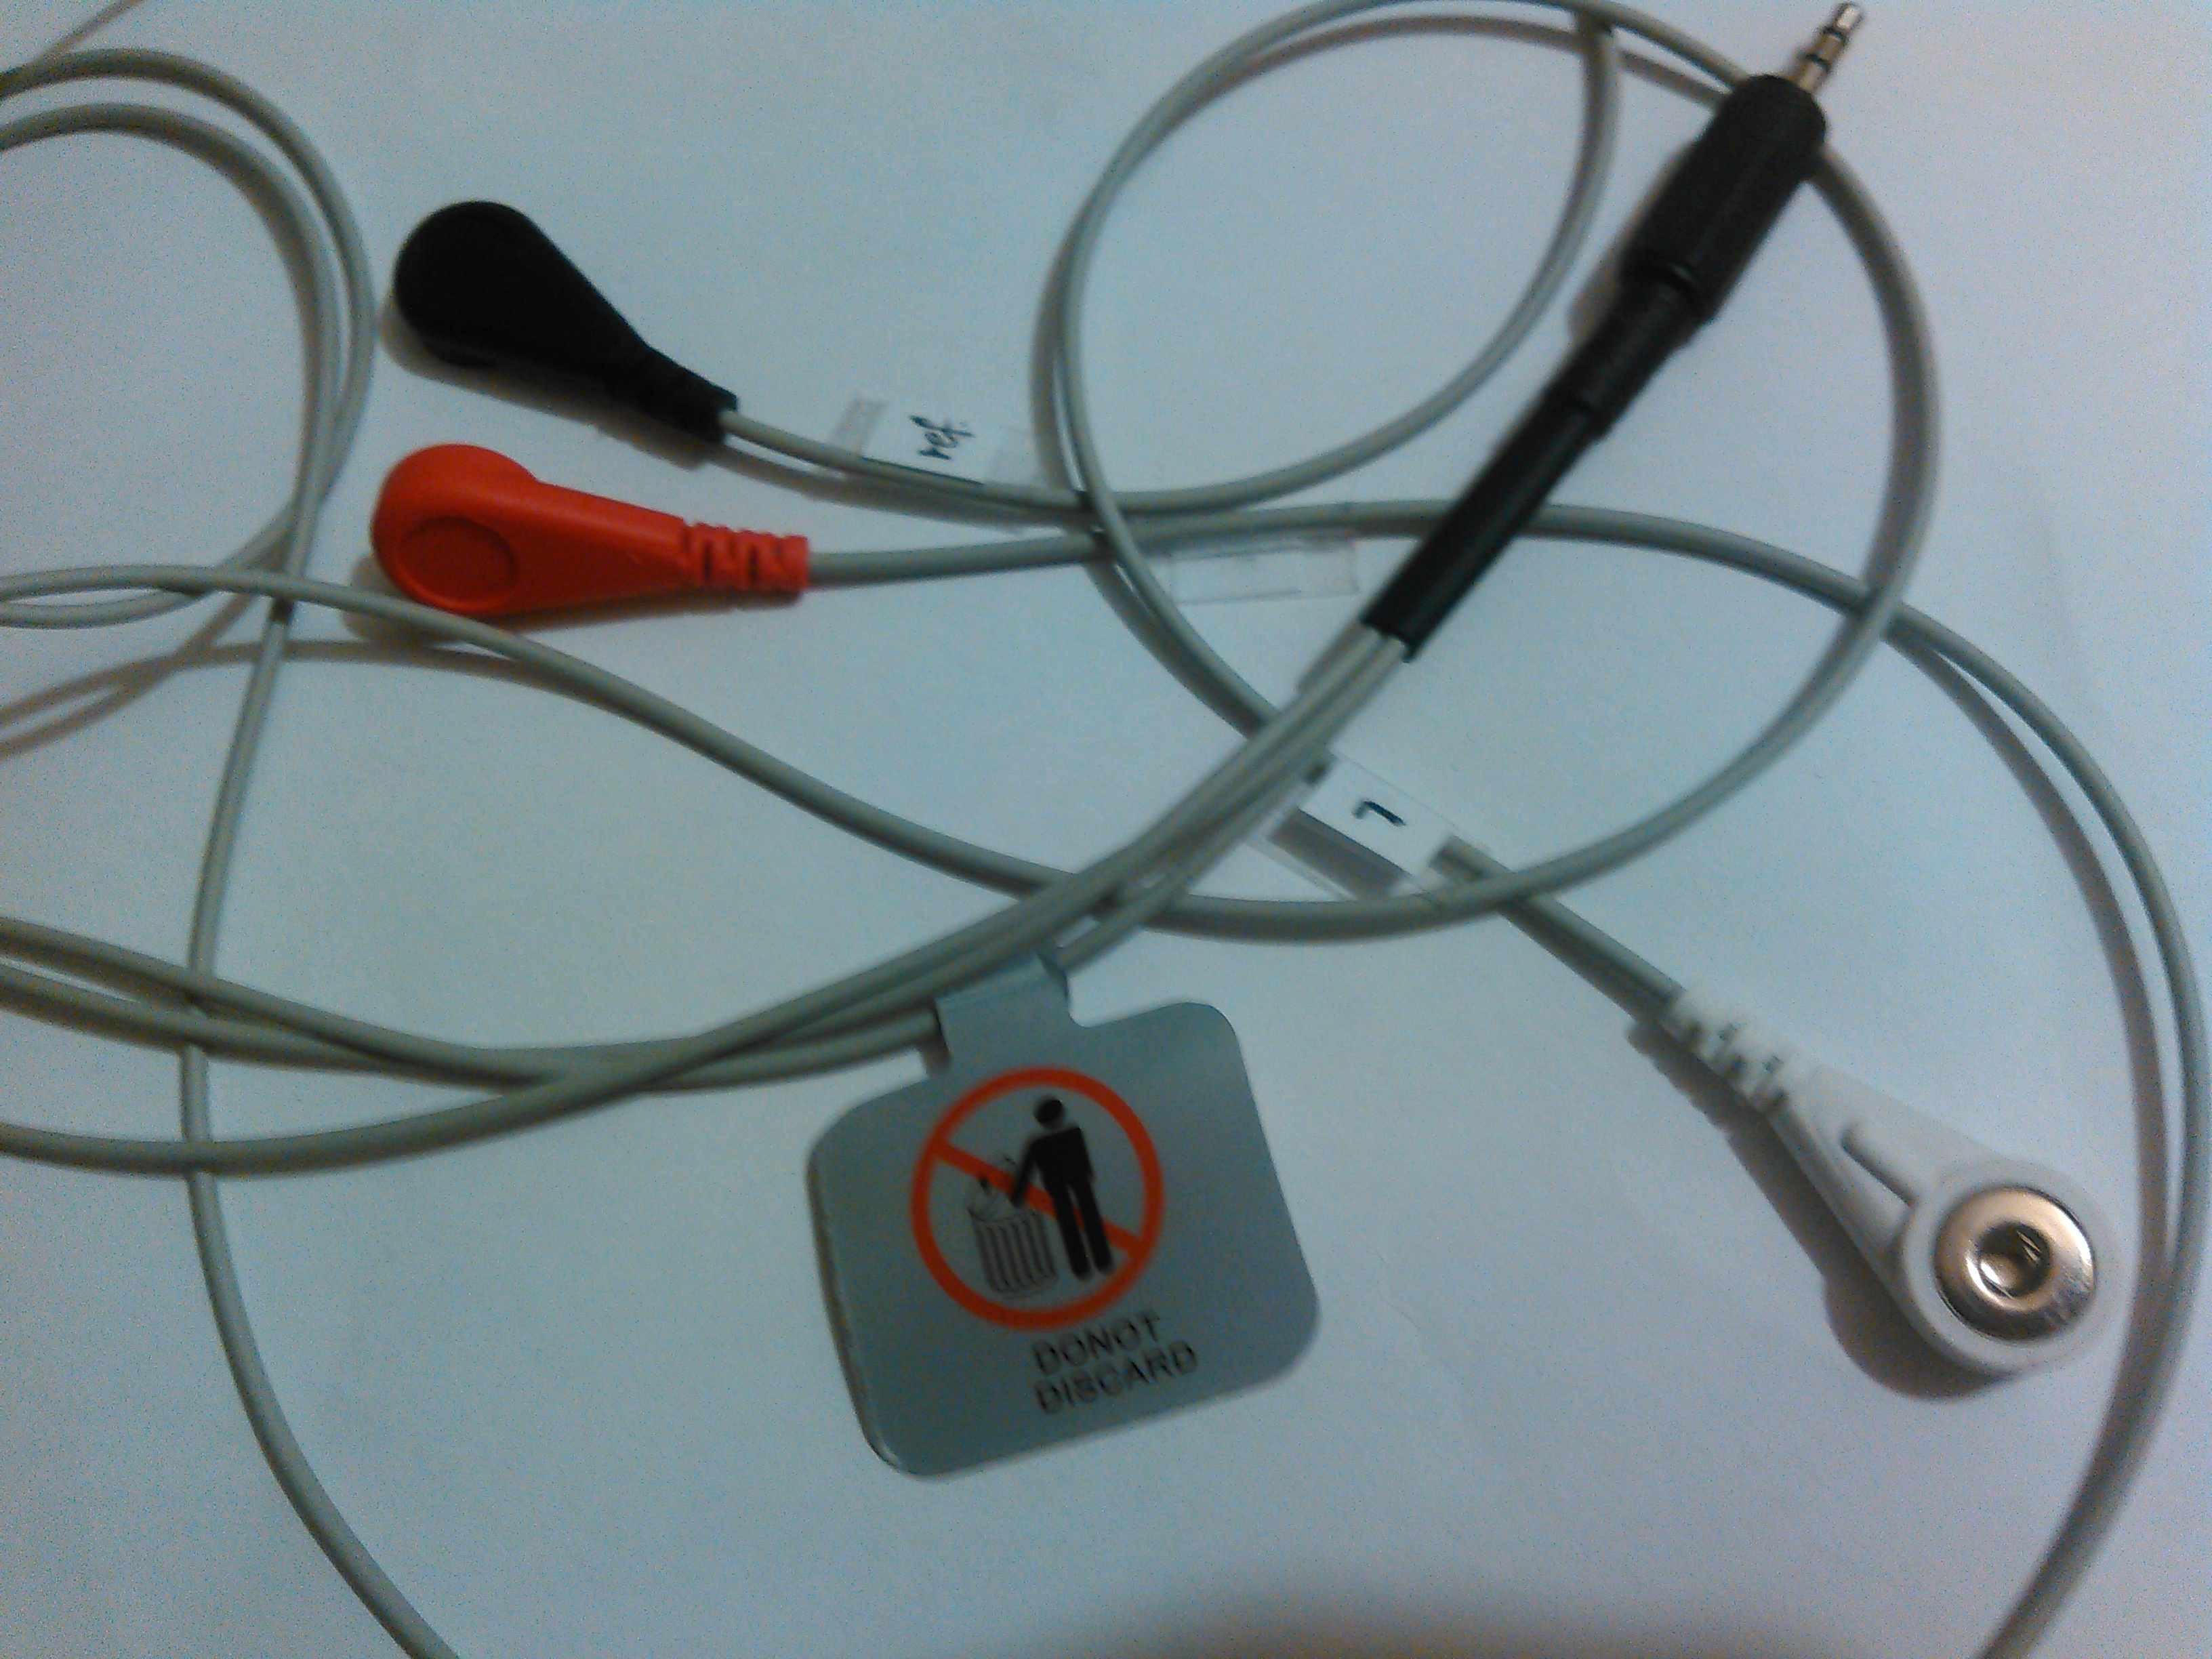
\includegraphics[width=0.8\textwidth]{24}
	\end{center}
    \caption{Lead}
	\label{fig:37}
\end{figure}
\begin{figure}[H]
	\begin{center}
		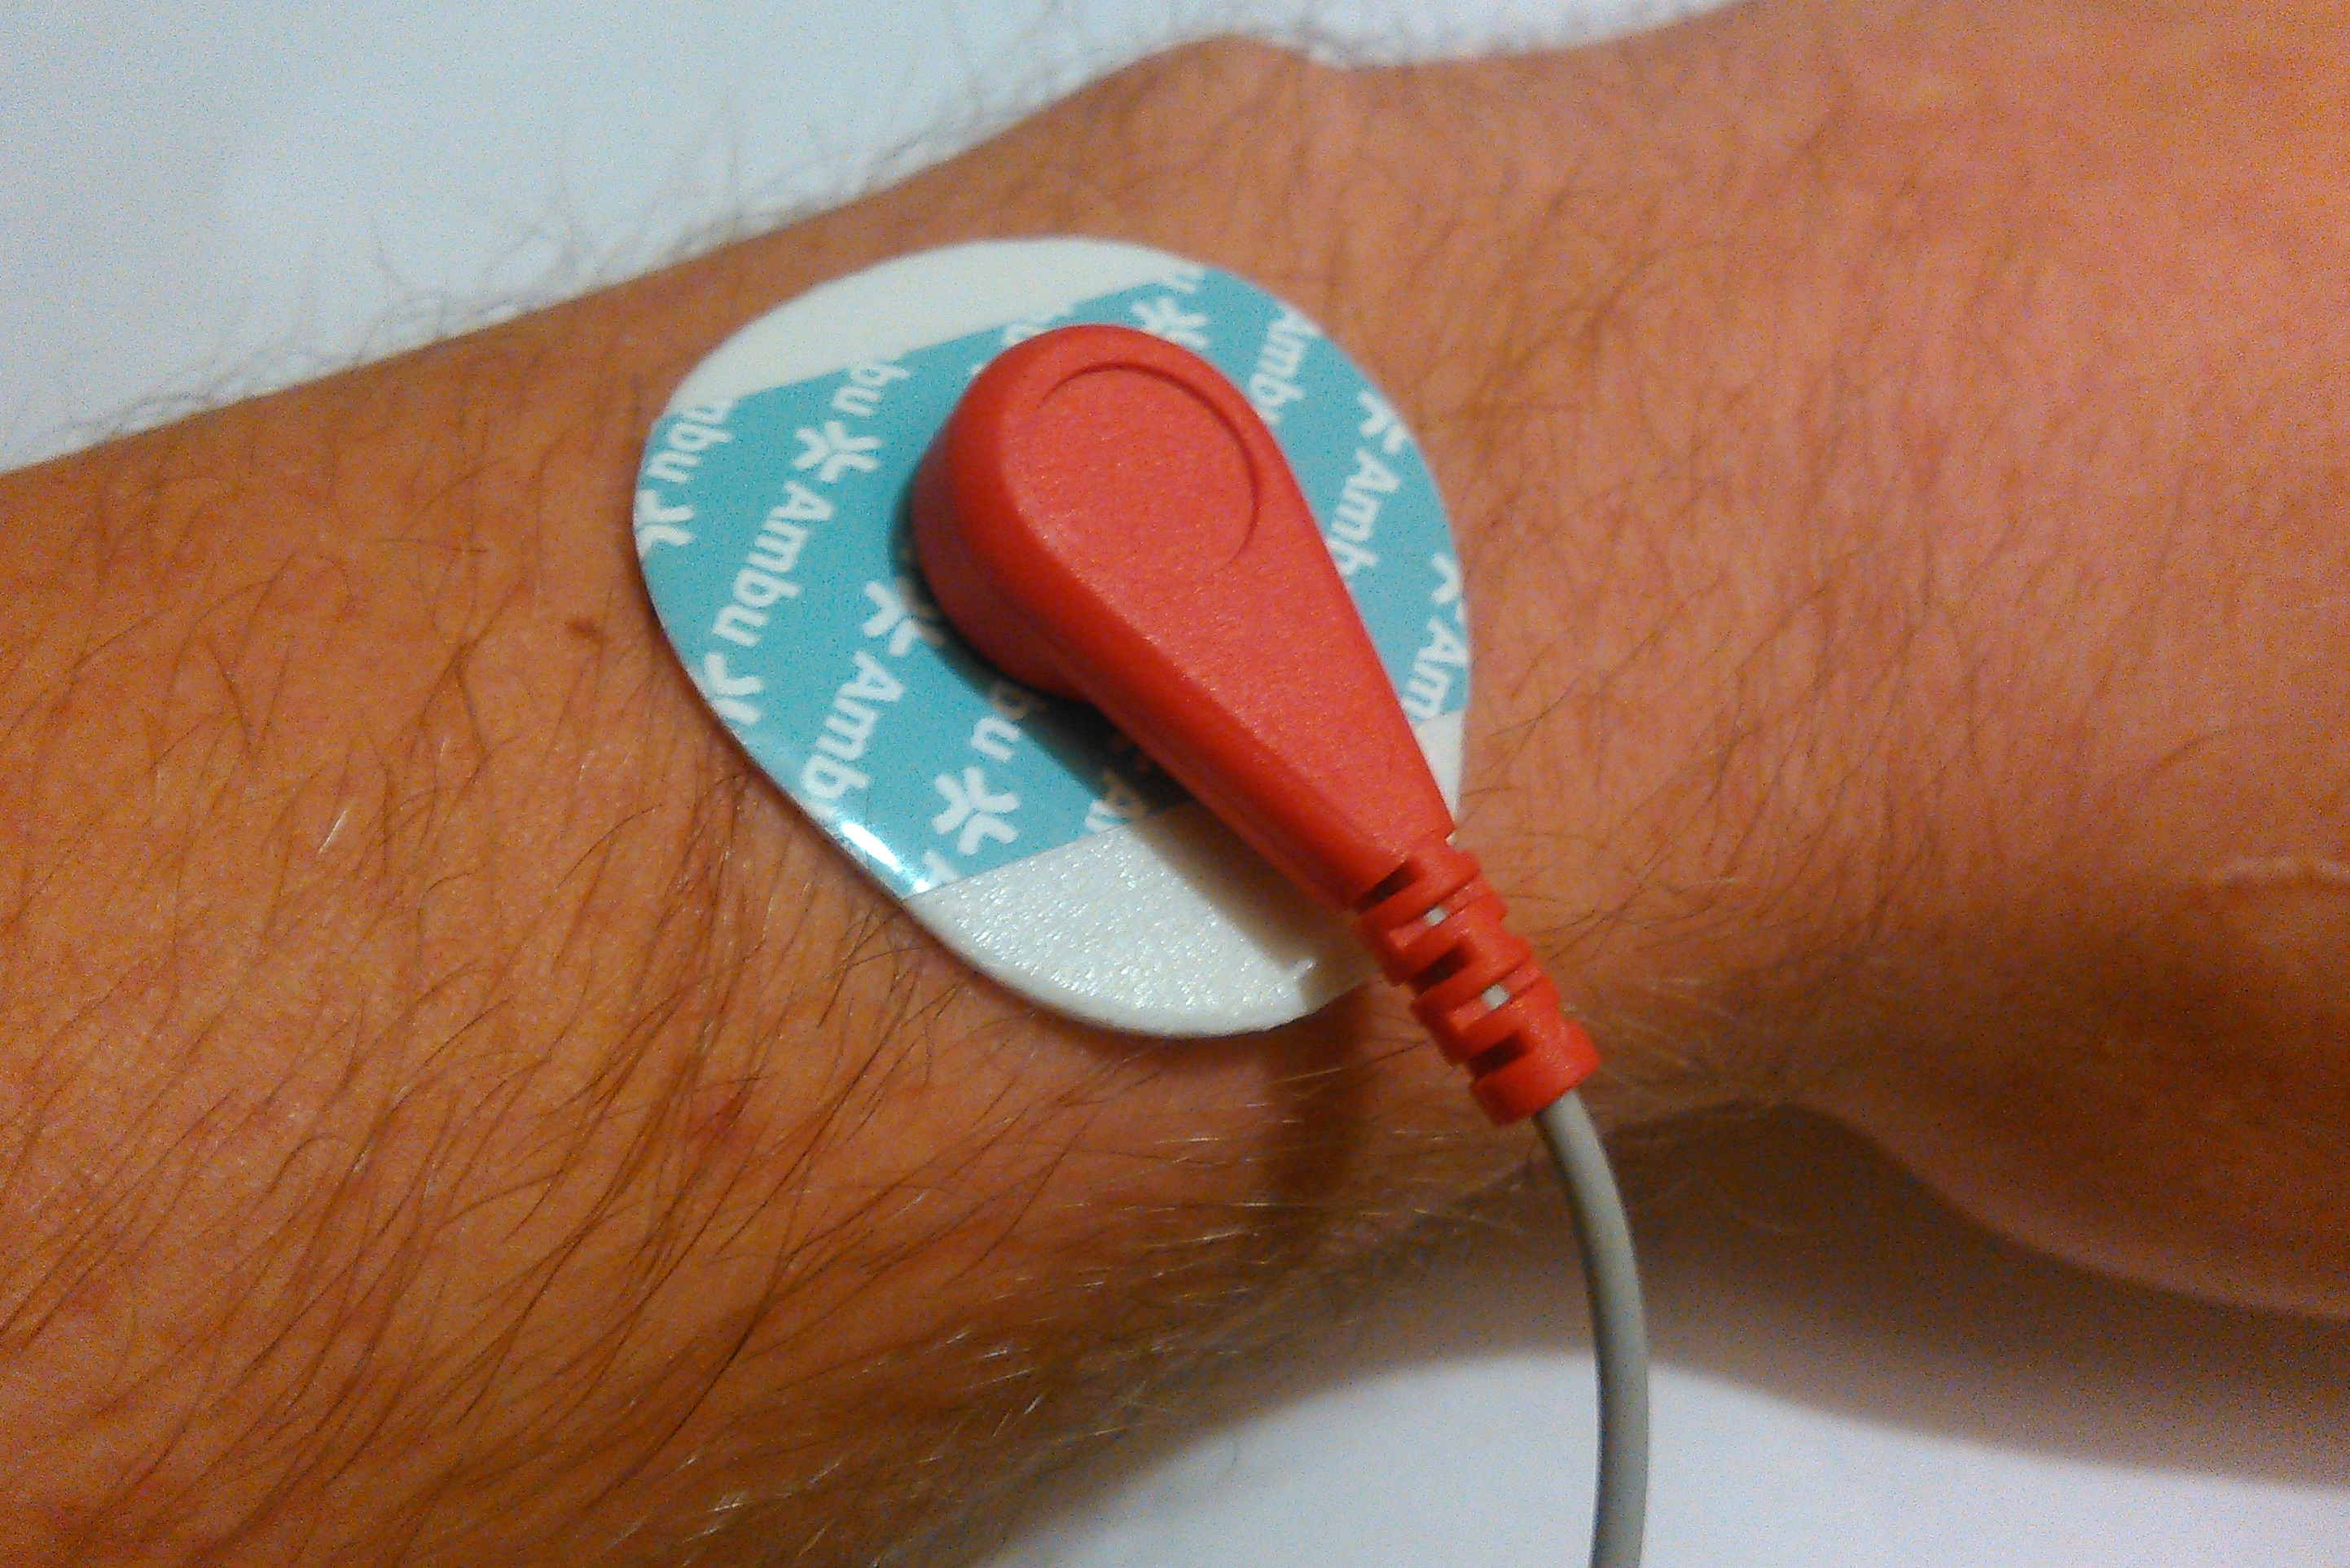
\includegraphics[width=0.8\textwidth]{25}
	\end{center}
    \caption{Electrode attached to the lead}
	\label{fig:38}
\end{figure}
Connect the Ethernet shield via a Ethernet cable to a router. Next turning the power button on the bread board power supply to power on the wearable device. This concludes the wearable device set-up.\\
To display the gathered data open the solution and run the program, see figure \ref{fig:18} on page~\pageref{fig:18} what the data display looks like.
\newpage
\section{Testing and Results}
Figures \ref{fig:27}, \ref{fig:39} show the A0 Olimex SHIELD-EKG-EMG value against time graph. Figure \ref{fig:27} with the highest possible sampling rate and figure \ref{fig:39} with the sampling rate of 200Hz. This shows that the sampling rate has been chosen correctly and as no crucial data has been lost. The noise could be caused by high frequency muscle contraction or power line interference (50Hz). Olimex SHIELD-EKG-EMG has a 3rd odder "Besselworth" filter with the cut-off frequency  set to 40Hz.
\begin{figure}[H]
	\begin{center}
		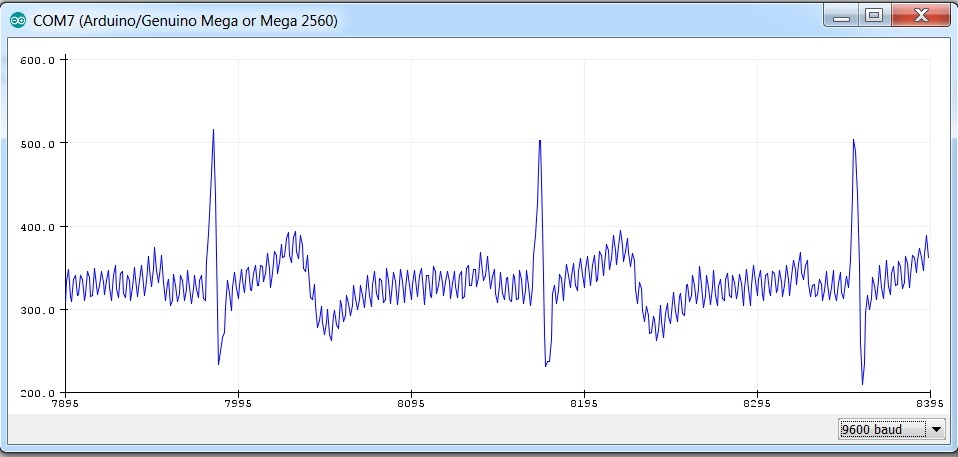
\includegraphics[width=0.8\textwidth]{26}
	\end{center}
    \caption{ECG with the highest possible sampling rate}
	\label{fig:27}
\end{figure}
\begin{figure}[H]
	\begin{center}
		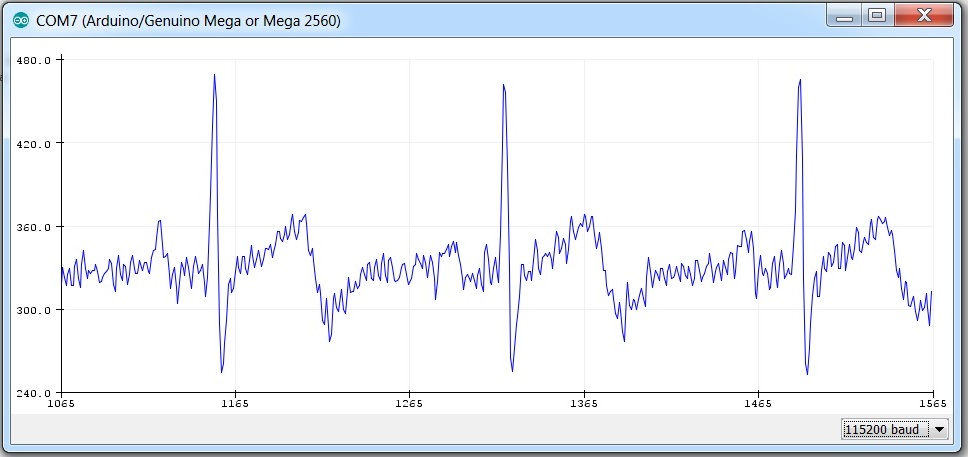
\includegraphics[width=0.8\textwidth]{27}
	\end{center}
    \caption{ECG with 200Hz sampling rate}
	\label{fig:39}
\end{figure}
Next the ECG signal of a stationary person (figure \ref{fig:27}), is compared to a physically active one (figure \ref{fig:40}), a conclusion can be drawn that collecting ECG data while the patient is walking results in the signal being very distorted. This limits the use of this very much as only one variable can be collected at a time. Either pedometer data is collected and the ECG data is too distorted, or the patient is forced to stay stationary.
\begin{figure}[H]
	\begin{center}
		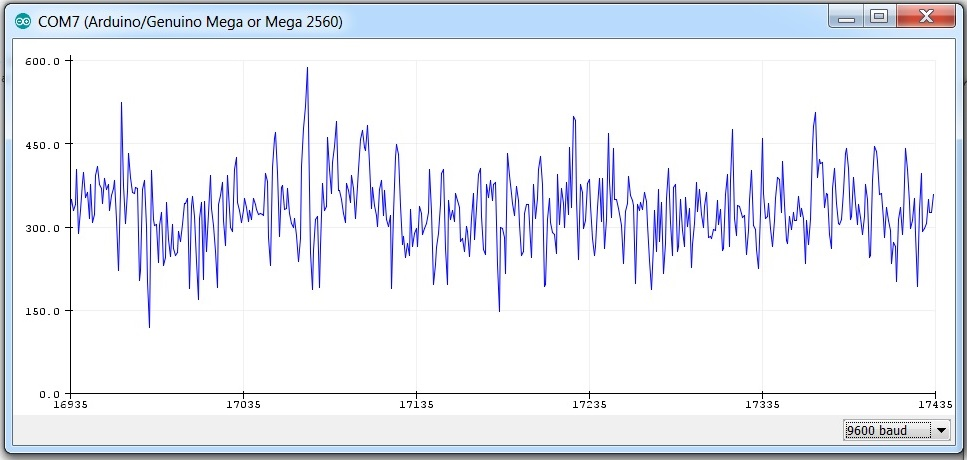
\includegraphics[width=0.8\textwidth]{28}
	\end{center}
    \caption{Active}
	\label{fig:40}
\end{figure}
All other data processing and data transferring steps work well as can be seen by figure \ref{fig:18} on page~\pageref{fig:18}. 
\section{Summary and Conclusion}
\textbf{To summarise} 
\begin{itemize}
\item[1] A wearable device capable of collecting ECG data and counting the patients steps (pedometer) has been successfully implemented.
\item[2] The device is also capable of sending this data to a remote database.
\item[3] A system of collecting the data and writing it to the database has been implemented successfully.
\item[4] A database to store the patients data has been designed.
\item[5] A web application having access to the database and capable of displaying the data has been built.
\end{itemize}
Therefore all project aims have been met. But some key design specifications have not. These are: 
\begin{itemize}
\item[1] The wearable device is not a mobile device because it requires constant Ethernet cable connection for the data to be sent to the database,
\item[2] The wearable device is not capable of sustaining long pedometer readings as the cables used for communication between the micro-controller and ADXL345 tend to come out and this stops the algorithm from functioning properly,
\item[3] The web application displays the data in a very raw manner, and is not intuitive.
\end{itemize}
To improve the project a voltage stabiliser should be used to provide sufficient power to the ESP8266 Wi-Fi module to work without rebooting. Another solution would be to use a Wi-Fi shield capable of running of 5V input. This will allow the patient to move freely with the device anywhere. Data saving to a SD card should be implemented. This will allow for data storage in case there is no internet available or the server is off-line for maintenance. A crucial improvement to the project is the permanent soldering of cable connections, used for supplying power and communication. This will result in more resilient wearable device. Another key feature of the project is the web application. Improving the application by displaying data as graphs, implementing user authentication that would allow several users to access their data would drastically improve project quality.
\newpage
\begin{thebibliography}{9}
\bibitem{Arduino} 
\textit{Arduino} MEGA 2560 and Ethernet Shield product page page: 
\\\texttt{https://store.arduino.cc/arduino-mega-2560-rev3}
\\\texttt{https://store.arduino.cc/arduino-ethernet-rev3-without-poe}
\\(Accessed on 2018/01/26)
 
\bibitem{Raspberry Pi} 
\textit{Raspberry Pi} 3 model B product page:
\\\texttt{https://www.raspberrypi.org/products/raspberry-pi-3-model-b/}
\\(Accessed on 2018/01/26)

\bibitem{KFI} 
Lincoln Cushing.
\textit{Kaiser Permanente and NASA – Taking Telemedicine Out of this World}. 
\\Heritage writer, September 2015

\bibitem{FCC} 
Federal Communication Commission.
\textit{Connecting America: The National Broadband Plan. The National Broadband Plan}. 
\\Washington, DC, USA, 2010

\bibitem{GEH}
\textit{ApexPro CH Telemetry System} product page:
\\\texttt{http://www3.gehealthcare.com/en/Products/Categories/Patient\_Monitoring/\newline Wireless\_Networks/ApexPro\_CH\_Telemetry\_System}
\\(Accessed on 2018/01/26)

\bibitem{BIO}
\textit{BIOTRONIK} official home page:
\\\texttt{https://www.biotronik.com/pl-pl}
\\(Accessed on 2018/01/26)

\bibitem{BOS}
\textit{LATITUDE™ NXT} product page:
\\\texttt{http://www.bostonscientific.com/en-US/products/remote-patient-monitoring\newline /latitude.html}
\\(Accessed on 2018/01/26)

\bibitem{AND}
\textit{A\&D} WellnessConnected products page:
\\\texttt{http://site.wellnessconnected.com/products/}
\\(Accessed on 2018/01/26)
\end{thebibliography}
\textbf{List of used software:}
\begin{itemize}
\item Arduino,
\item Win32DiskImager,
\item PuTTY,
\item Raspberrian Jessie,
\item MariaDB,
\item Apache,
\item MySQL,
\item Visual Studio,
\item LaTeX.
\end{itemize}
The licences for the software can be found in the '/Raport/License/' directory.
\end{document}
